\chapter{Viento a 10 metros}\label{cap:resultados_wind10}

En los ciclones extratropicales, el viento en superficie es un forzante dinámico que transfiere momento continuo al océano, modulando la formación de oleaje anómalo \citep{gramcianinov2023impact}.
La severidad física de estos sistemas ha sido documentada por \citet{bartolomei2024extremos}, quienes caracterizan la extrema actividad cinemática generada por ciclones invernales en el sur de Brasil. 
Además, modelaciones climáticas de alta resolución proyectan que el calentamiento global intensificará el sector cálido de estos ciclones, incrementando los vientos y la precipitación en sus etapas de desarrollo \citep{gentile2025response}; para las tres zonas de ciclogénesis del Atlántico Sudoccidental, esta intensificación se proyecta en hasta 1.5--2~m\,s$^{-1}$ en los vientos de niveles bajos hacia fines de siglo, pese a una disminución proyectada en la frecuencia de ciclogénesis \citep{dejesus2021multimodel}. Esta proyección es asimétrica en su nivel de certeza: el IPCC atribuye alta confianza al aumento de las tasas de precipitación asociadas a estos sistemas, pero solo confianza media a los cambios en su intensidad dinámica (viento) \citep{IPCC2021_WG1_Chapter11_Extremes}.

El campo de viento a 10 metros integra forzantes de múltiples escalas: desde flujo de gran escala hasta fenómenos mesoescalares como chorros de bajo nivel, descargas descendientes y seclusiones térmicas (véase Sección~\ref{subsec:tb_modelos}). 
La población de ciclones abarca desde sistemas débiles —cuyo viento responde al flujo de fondo— hasta vórtices intensos que desarrollan asimetrías complejas con núcleos de velocidad máxima en sectores específicos de sus cuadrantes.

El presente capítulo busca establecer la estructura espacial del viento a 10 metros durante el ciclo de vida de los ciclones extratropicales del Atlántico Sudoccidental y su límite con Sudamérica. 
Específicamente, se busca: (i)~cuantificar la evolución de las distribuciones de magnitud del viento según la intensidad dinámica del sistema y su región de génesis; (ii)~determinar la localización espacial preferencial de los máximos de viento en un sistema de coordenadas relativo al centro del ciclón; y (iii)~descomponer la estructura espacial de la variabilidad del viento para identificar patrones dominantes y su evolución estadística durante las fases.

El análisis se estructura siguiendo una progresión desde la descripción estadística hacia la comprensión dinámica. 
La Sección~\ref{sec:pdf_wind10} examina las funciones de densidad de probabilidad (PDF) de las magnitudes máximas, estableciendo diferencias entre el comportamiento medio de ciclones y los intensos (p90); véase también Sección~\ref{subsec:subconjuntos_intensidad}). 
Las Secciones~\ref{sec:kde_espacial_global} y~\ref{sec:kde_espacial_p90} analizan la distribución de probabilidad de posición (PDFe) de estos máximos mediante estimaciones de densidad kernel (KDE; Sección~\ref{subsec:kde_localizacion}), contrastando la dispersión característica de la población general contra la organización hiperconcentrada observada en p90. 
Finalmente, las Secciones~\ref{sec:var_exp_wind10}--\ref{subsec:res_dinamica_pc1} emplean funciones ortogonales empíricas (EOF; Sección~\ref{subsec:eof_univariado}) para descomponer la estructura modal de la variabilidad del viento.

Los hallazgos de este capítulo se complementarán con el análisis del campo de precipitación (Capítulo~\ref{cap:resultados_tp}), para posteriormente en el Capítulo~\ref{chap:meof} explorar si la distribución espacial de los máximos de viento y precipitación no necesariamente coinciden, respondiendo a mecanismos físicos diferenciados dentro de la estructura del ciclón, aspecto introducido en la Sección~\ref{subsec:tb_compound_def}.

% --- SECCIÓN PRINCIPAL: PDF DE VIENTO A 10 METROS ---

\section{Distribución de magnitudes (PDF)}\label{sec:pdf_wind10}

La Figura~\ref{fig:pdf_wind10} presenta las funciones de densidad de probabilidad que describen la distribución estadística de los máximos de viento en superficie a 10~metros. 
Estos valores fueron extraídos del dominio lagrangiano centrado en el núcleo de vorticidad, siguiendo el procedimiento detallado en la Sección~\ref{subsec:extraccion_pdf}, sobre la base de las dos poblaciones de estudio construidas en la Sección~\ref{sec:poblaciones_estudio}. 
La muestra se encuentra estratificada por región de ciclogénesis (SBR, LPB, ARG; Sección~\ref{sec:tb_regiones}) y se evalúa a lo largo de las cuatro fases de desarrollo (Ic, It, M, D; Sección~\ref{subsec:tb_fases}), contrastando la Población Global contra el subconjunto p90.

Durante la fase incipiente (Ic; paneles a, b y~c), tanto la Población Global como el subconjunto p90 presentan distribuciones unimodales parcialmente superpuestas, con frecuencias máximas concentradas en el rango de 10 a 17~m\,s$^{-1}$. A medida que los sistemas evolucionan hacia las fases de intensificación (It; paneles d, e y~f) y madurez (M; paneles g, h e~i), se hace evidente la divergencia entre los grupos: la curva del subconjunto p90 se desplaza hacia la derecha, alcanzando en la fase~M un pico en el rango de 20 a 22~m\,s$^{-1}$ y colas extendiéndose hasta los 30~m\,s$^{-1}$, mientras que la Población Global mantiene su máximo alrededor de los 12--15~m\,s$^{-1}$ con una distribución más estrecha y simétrica. Regionalmente, en la etapa de madurez de SBR (g), el p90 exhibe un pico de densidad (${\sim}0.18$) acotado en altas velocidades; LPB (h) presenta igualmente un desplazamiento hacia velocidades mayores, aunque con un pico más bajo y distribución más extendida (${\sim}0.07$), mientras que ARG (i) muestra la distribución más ancha y aplanada de las tres regiones, evidenciando una mayor heterogeneidad en la intensidad de sus sistemas. Finalmente, en la fase de decaimiento (D; paneles j, k y~l), las curvas del subconjunto p90 retroceden hacia magnitudes menores y aumentan su dispersión, preservando no obstante una separación inconfundible respecto a los sistemas más débiles.

\begin{figure}[htbp]
\centering
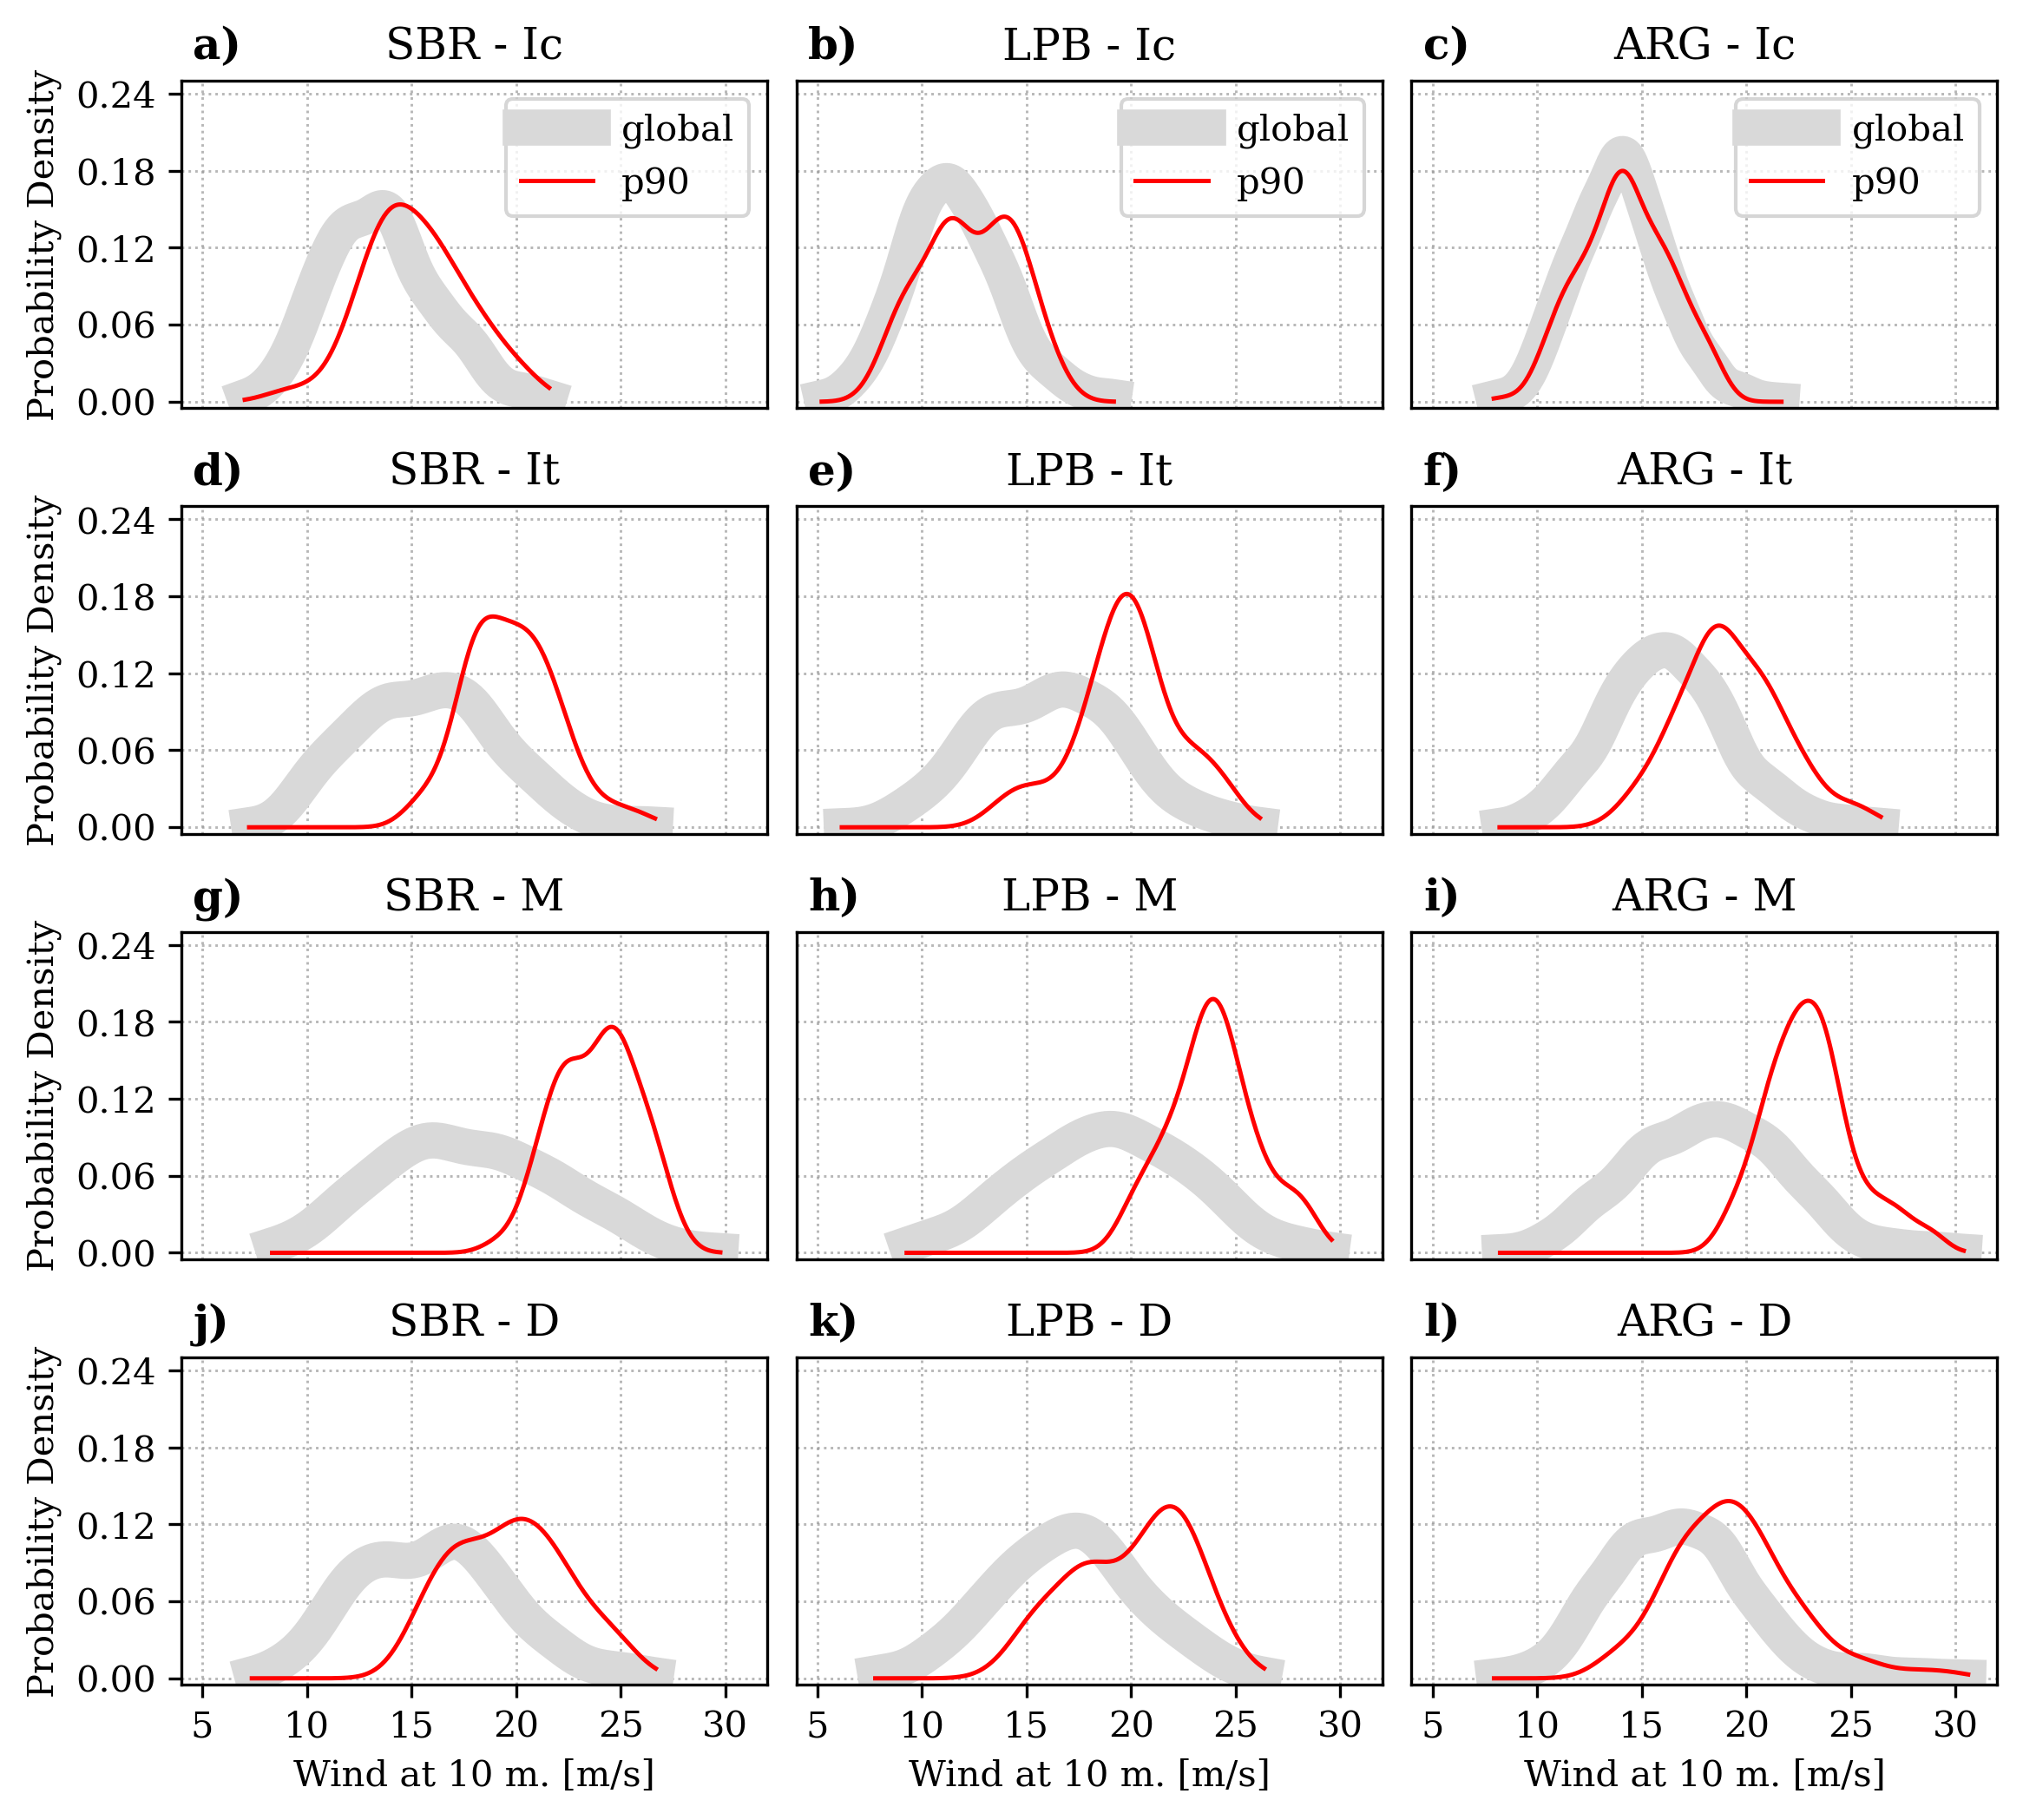
\includegraphics[width=\textwidth]{images/w10/PDF_wind10_sigma025.png}
\caption[PDF de magnitudes máximas de viento a 10 metros]{Funciones de densidad de probabilidad (PDF) para las magnitudes máximas de viento a 10 metros. Las columnas indican la región de ciclogénesis (SBR, LPB, ARG) y las filas la evolución a través de las fases del ciclo de vida (Ic, It, M, D). Se contrasta la población global (referencia, sombreado gris) con los subconjuntos definidos por percentiles de los máximos de vorticidad relativa en 850~hPa alcanzados en su ciclo vital: p90 (sistemas intensos, línea roja).}
\label{fig:pdf_wind10}
\end{figure}

La máxima separación de las distribuciones en la fase de madurez refleja el momento en que los ciclones intensos (p90) expresan su pleno potencial dinámico, alcanzando su mínimo absoluto de vorticidad relativa a 850~hPa y maximizando el gradiente horizontal de presión superficial, comportamiento coherente entre la población global y el subconjunto p90 presentada en la Tabla~\ref{tab:fase_max_intensidad}. 
La diferencia respecto a la Población Global es que desde su génesis su entorno es más inestable y esto culmina en campos de viento más severos que el desarrollo estándar.

Las variaciones interregionales reflejan distintos forzamientos físicos predominantes. 
Tal como sostiene \citet{gramcianinov2024early}, los sistemas en las regiones SBR y LPB alcanzan intensidades de viento más extremas debido a la influencia de procesos termodinámicos en niveles bajos, como la advección cálida y la convergencia de humedad (véase Sección~\ref{subsec:tb_sbr} y Sección~\ref{subsec:tb_lpb}).
Esta dependencia termodinámica es respaldada por \citet{gozzo2013air}, quienes demostraron que los flujos turbulentos de calor sensible y latente océano-atmósfera, acoplados a una profunda inyección de humedad, son mecanismos decisivos para desestabilizar el entorno y retroalimentar el sistema en desarrollo.
Este aspecto termodinámico es analizado por \citet{russo2025impacts}, quienes sostienen que, si bien la ciclogénesis inicial depende de procesos dinámicos de niveles altos, la inyección masiva de humedad y flujos de calor latente resulta fundamental durante las fases de intensificación y madurez.
En la costa del sur y sudeste de Brasil, \citet{rocha2016estudio} muestran además que la difluencia en altura, un cavado en niveles medios y, especialmente, la convergencia en bajos niveles favorecen la ciclogénesis regional.

Mientras tanto, en ARG, la dinámica baroclínica clásica del frente y la perturbación topográfica de los Andes generan respuestas cinemáticas más variables y distribuciones más aplanadas (Sección~\ref{subsec:tb_arg}). 
De acuerdo con \citet{gan1994influence}, la interacción con la orografía induce distorsiones espaciales en el flujo de niveles bajos y modifica la estructura de las ondas \citep{vera2002cold}. Este entorno está fuertemente condicionado por la baroclinicidad ambiental y los gradientes térmicos horizontales \citep{yanase2014parameter}, proceso intrínsecamente ligado a la incursión de anomalías de vorticidad potencial en niveles altos durante la ciclogénesis en el este continental \citep{crespo2020potential, gramcianinov2019properties}.

La cuantificación de estas distribuciones permite comparar cómo evolucionan las magnitudes más probables y la extensión de los valores entre ciclones de distinta génesis. 
Al confirmar que los ciclones clasificados dinámicamente como intensos (p90) se separan sistemáticamente de la población a medida que maduran, se valida la clasificación basada en vorticidad, descrita en la Sección~\ref{sec:poblaciones_estudio}. 
En la fase de madurez, p90 desplaza su mayor probabilidad hacia los $\sim$23~m\,s$^{-1}$ (Figura~\ref{fig:pdf_wind10}, paneles g--i), lo que representa un incremento de aproximadamente el 50\% respecto a la moda de la Población Global ($\sim$15~m\,s$^{-1}$).

Las colas en las distribuciones p90 alcanzan magnitudes de hasta 30~m\,s$^{-1}$. 
Este corrimiento coincide con los registros documentados por \citet{padilhareinke2026characterization}, \citet{cardoso2022synoptic} y \citet{gramcianinov2020analysis} para los eventos severos del Atlántico Sur, y especificamente para SBR coincide con \citet{gozzo2014subtropical} en ciclones subtropicales.
\citet{padilhareinke2026characterization} reportan una intensidad media de viento a 10~metros de 70.0~km\,h$^{-1}$ (${\approx}$\,19.4~m\,s$^{-1}$), con un umbral para eventos intensos p90 de 84.4~km\,h$^{-1}$ (${\approx}$\,23.4~m\,s$^{-1}$) y magnitudes extremas que alcanzan hasta 113.21~km\,h$^{-1}$ (${\approx}$\,31.4~m\,s$^{-1}$) en las colas de la distribución. 
Estos rangos son consistentes con lo documentado por \citet{gramcianinov2020analysis}, quienes reportan, para el invierno austral (JJA), velocidades máximas medias de 21.2\,$\pm$\,4.8~m\,s$^{-1}$ (percentil~90: 27.3~m\,s$^{-1}$; percentil~95: 29.3~m\,s$^{-1}$) en ERA5, y de 23.4\,$\pm$\,4.8~m\,s$^{-1}$ (percentil~90: 30.2~m\,s$^{-1}$; percentil~95: 32.1~m\,s$^{-1}$) en CFSR/CFSv2.
Asi mismo \citet{corner2025classification}, empleando un método de clasificación de ciclones distinto en el Hemisferio Norte, identifican que el grupo de los ciclones más débiles presenta una moda en la velocidad del viento a 10~metros de 12.5~m\,s$^{-1}$, mientras que los ciclones más intensos alcanzan los 22.5~m\,s$^{-1}$.
Como subraya \citet{gramcianinov2023impact}, identificar tempranamente sistemas intensos resulta indispensable, ya que estos vientos anómalos son los forzantes para eventos asociados que suponen un riesgo directo para las regiones costeras y marítimas.


% --- SECCIÓN PRINCIPAL: KDE ESPACIAL DE VIENTO A 10 METROS ---

\section{Distribución espacial de máximos (PDFe)}
\subsection{Población Global}\label{sec:kde_espacial_global}

\begin{figure}[htbp]
\centering
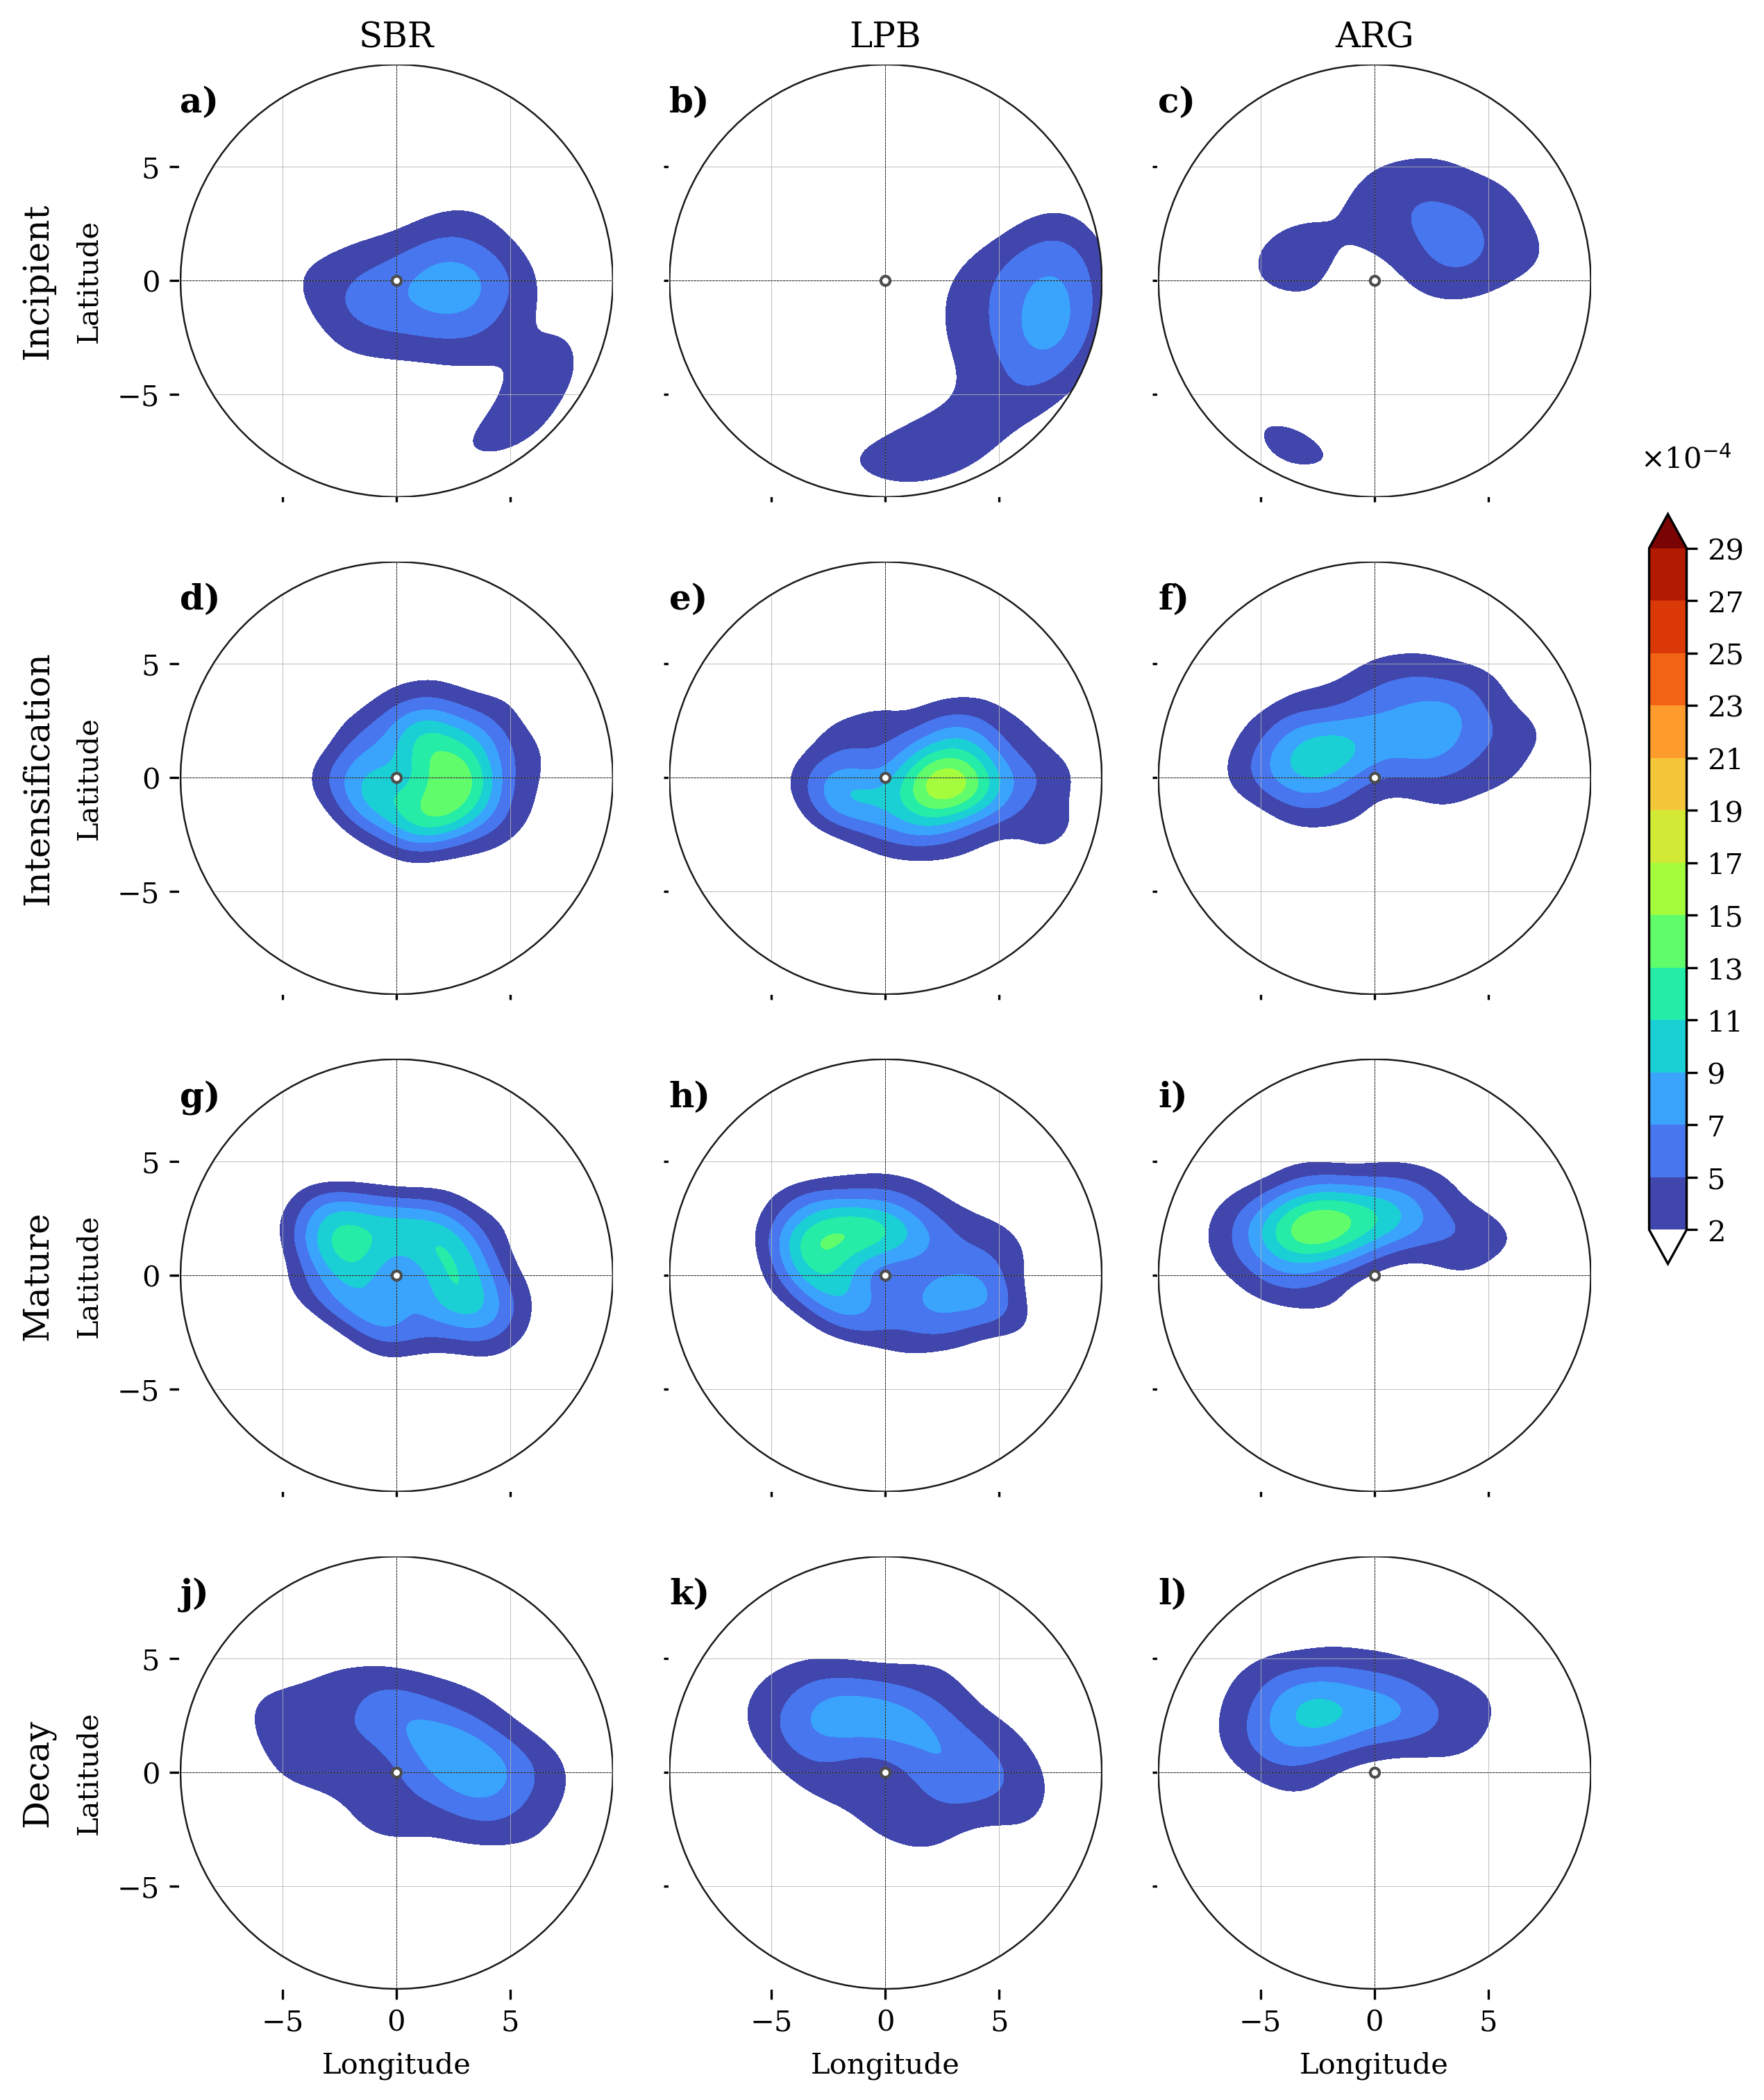
\includegraphics[width=\textwidth]{images/w10/kde_wind10_global_fasesxreg.png}
\caption[PDF espacial de viento máximo a 10 metros --- Población Global]{Estimación de densidad espacial bidimensional (PDFe; Sección~\ref{subsec:kde_localizacion}) de la ubicación de los máximos de magnitud de viento a 10~metros para la Población Global. Las columnas separan las regiones de ciclogénesis (SBR, LPB, ARG) y las filas indican las fases evolutivas (Ic, It, M, D). El dominio lagrangiano está centrado en el ciclón ($0^{\circ}, 0^{\circ}$).}
\label{fig:kde_wind_global}
\end{figure}

La Figura~\ref{fig:kde_wind_global} presenta el campo de densidad espacial sobre el dominio lagrangiano de $20^{\circ} \times 20^{\circ}$ definido en la Sección~\ref{sec:procesamiento_lagrangiano}. 
En términos generales, la distribución se caracteriza por ser amplia, difusa y con gradientes de probabilidad suaves, sin que ninguna fase o región exhiba una concentración extrema comparable a la que se documenta en los sistemas p90. 
Esta dispersión es la firma esperada de una población heterogénea que abarca desde sistemas débiles hasta configuraciones atípicas, comportamiento documentado para el Hemisferio Sur por \citet{simmonds2000mean} y coherente con los métodos basados en vorticidad de \citet{sinclair1994objective}, lo que sugiere que se trata de un rasgo estructural de la climatología ciclónica y no de un efecto metodológico.

La evolución por fases revela una organización progresiva hacia el cuadrante noroeste. 
En las fases iniciales (Ic; paneles a, b y~c), las zonas de máxima densidad abarcan áreas extensas sin definir una estructura simétrica alrededor del centro ciclónico, coherente con la alta variabilidad en la intensidad de los sistemas descrita por \citet{reboita2010south} y con el comportamiento de génesis documentado por \citet{bartolomei2024extremos}, donde los sistemas suelen presentar circulaciones asimétricas antes de organizar un centro de baja presión cerrado y bien definido. 
Durante la fase de intensificación (It; paneles d, e y~f), las distribuciones muestran una transición hacia estructuras más compactas, con un aumento progresivo en la concentración de los máximos de viento hacia el cuadrante noroeste, consistente con el desarrollo de la circulación ciclónica documentado por \citet{gramcianinov2019properties}. 
En esta fase, LPB (e) presenta el núcleo de mayor densidad, alcanzando valores de ${\approx}$\,17--19\,$\times10^{-4}$, lo que sugiere una localización más recurrente de los vientos máximos durante el período de profundización; ARG (f), en cambio, exhibe una distribución más elongada en la dirección zonal, reflejando mayor dispersión en la posición del máximo de viento.
A medida que los sistemas avanzan hacia la madurez (M; paneles g, h e~i), se consolida el desplazamiento hacia el cuadrante noroeste, aunque con diferencias posicionales entre regiones que se discuten a continuación. 
En la fase de decaimiento (D; paneles j, k y~l), el núcleo asimétrico se mantiene en el sector noroeste, aunque con densidades menores y contornos más difusos respecto a la madurez, indicando una pérdida gradual de organización coherente con el debilitamiento del sistema.

El contraste regional más marcado se manifiesta en la fase de madurez. ARG (i) alcanza densidades de ${\approx}$\,17--19\,$\times10^{-4}$ concentradas en un único núcleo, mientras que SBR (g) y LPB (h) exhiben valores menores distribuidos en dos focos, firma de la estructura más variable que pueden presentar los sistemas en estas regiones. 
Como sugieren \citet{dossantos2023response} y \citet{yanase2014parameter}, esta evolución espacial asimétrica está ligada a las zonas baroclínicas donde los máximos gradientes térmicos horizontales interactúan con los chorros en la alta troposfera. En ARG, el patrón responde principalmente a la advección térmica y a la perturbación topográfica de los Andes; en SBR y LPB, en cambio, la mayor concentración se favorece por la advección de aire cálido y húmedo (Sección~\ref{sec:pdf_wind10}).

La dispersión observada en la población global refleja además la amplia variabilidad en la distancia al centro en la que ocurren los vientos máximos. 
En el Atlántico Sur, tanto \citet{gozzo2014subtropical} como \citet{cardoso2020wind} encuentran que los vientos máximos se ubican a una distancia del centro —entre 300-450~km y 400-500~km, respectivamente. 
Esta heterogeneidad justifica metodológicamente la estratificación por intensidad (Sección~\ref{subsec:subconjuntos_intensidad}): \citet{corner2025classification} y \citet{eisenstein2023identification} señalan que la diversidad estructural de estos sistemas exige aislar los eventos severos, práctica habitual en el Hemisferio Norte pero aún insuficientemente sistemática en el Hemisferio Sur. 
La organización geométrica de los sistemas intensos es examinada a continuación tomando esta población como línea base de referencia.

\subsection{Subconjunto de ciclones intensos p90}\label{sec:kde_espacial_p90}

\begin{figure}[htbp]
\centering
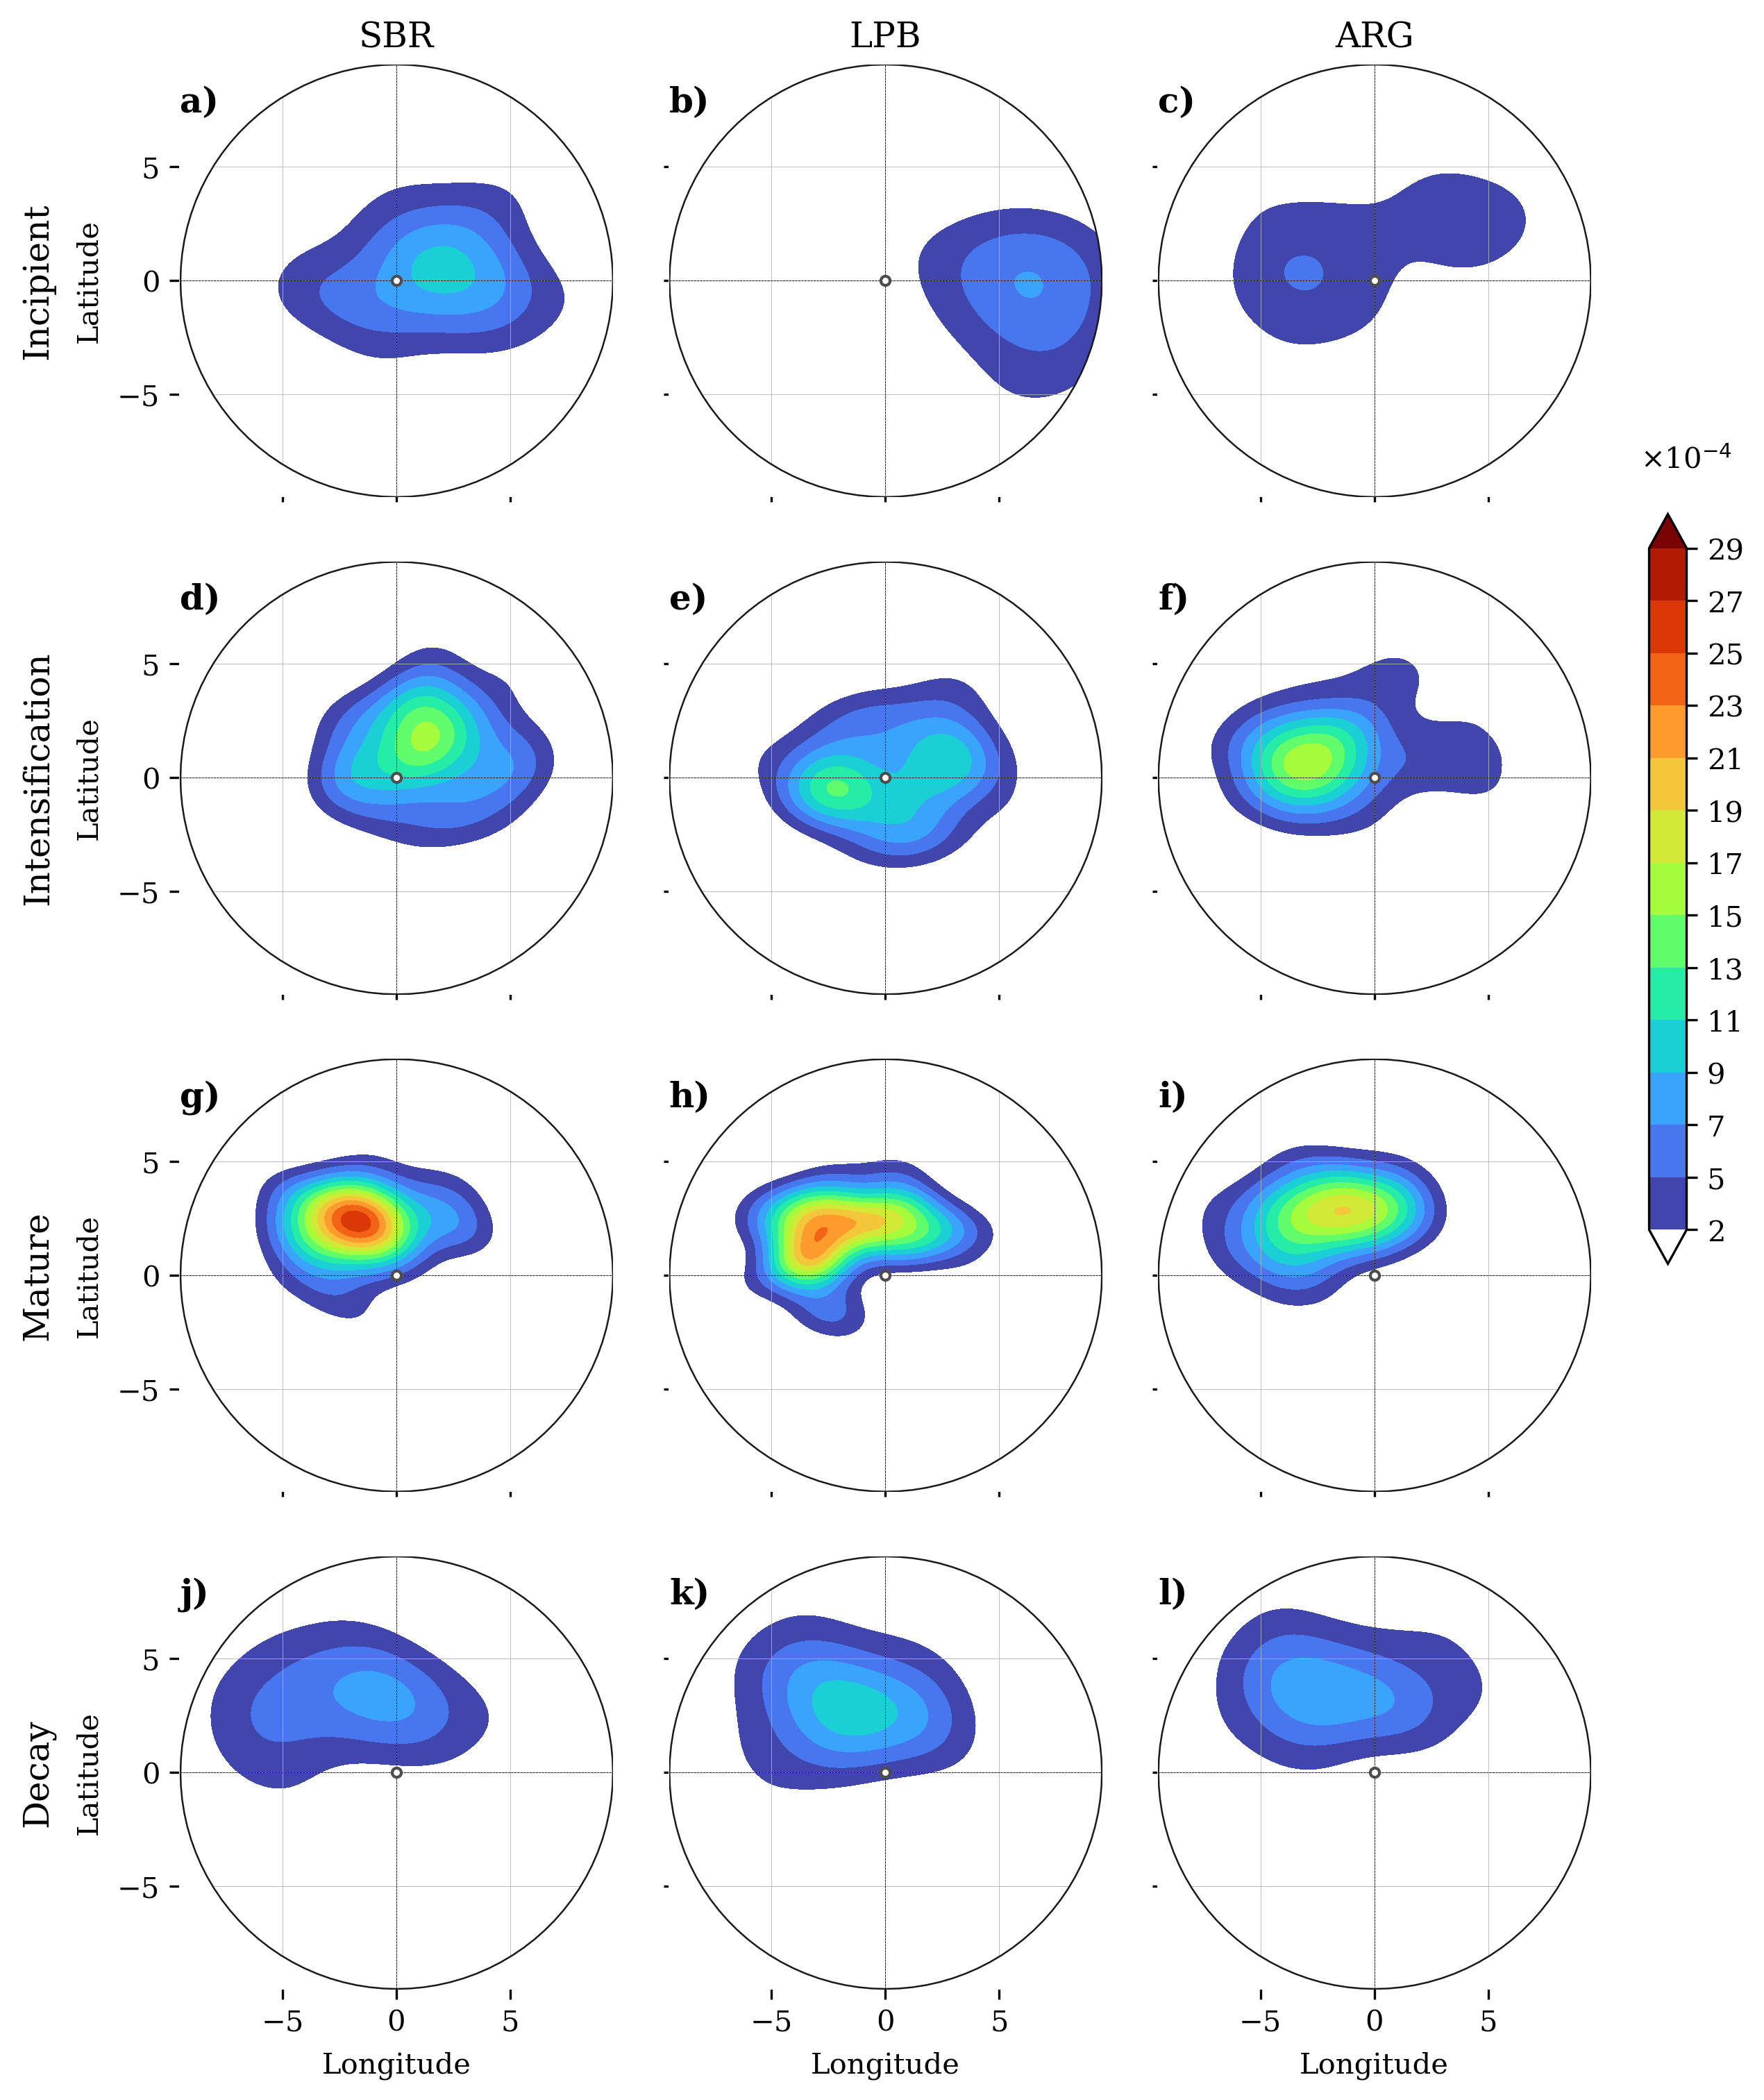
\includegraphics[width=\textwidth]{images/w10/kde_wind10_p90_fasesxreg.png}
\caption[PDF espacial de viento máximo a 10 metros --- Subconjunto p90]{Estimación de densidad espacial bidimensional (PDFe; Sección~\ref{subsec:kde_localizacion}) de la ubicación de los máximos de magnitud de viento a 10~metros para el subconjunto de ciclones intensos. El formato, dominio lagrangiano, fases evolutivas y escala de densidad ($10^{-4}$) son idénticos a los presentados en la Figura~\ref{fig:kde_wind_global} para permitir la comparación estructural directa de las asimetrías de densidad.}
\label{fig:kde_wind_p90}
\end{figure}

Al contrastar la línea base contra el subconjunto de sistemas intensos (p90), la reorganización espacial es marcada: la estructura de los vientos máximos deja de ser mayoritariamente difusa y comienza a consolidarse progresivamente en un cuadrante preferencial a medida que el sistema evoluciona. 
La Figura~\ref{fig:kde_wind_p90} documenta esta transición a lo largo de las cuatro fases evolutivas y para las tres regiones de ciclogénesis.

En las fases iniciales (Inc; paneles a, b y~c), las tres regiones mantienen una densidad baja y una zona de preferencia poco definida, comportamiento análogo al de la población global. 
A medida que los sistemas se intensifican (Int; paneles d, e y~f), los núcleos comienzan a desplazarse hacia el noroeste en SBR y LPB; en ARG (f), el foco de los máximos aumenta drásticamente respecto a la fase precedente, anticipando la concentración que caracterizará la madurez. 
El cambio más notorio ocurre en la fase de madurez (M; paneles g, h e~i): se configura un núcleo de alta densidad hiperconcentrado en el cuadrante noroeste, localizado aproximadamente a $-1^{\circ}$ a $-3^{\circ}$ de longitud y entre $+2^{\circ}$ y $+3^{\circ}$ de latitud relativa al centro.
Las magnitudes alcanzadas en SBR (g) son extremas (23--$27 \times 10^{-4}$), mientras que LPB (h) alcanza valores de ${\approx}$\,23--25\,$\times 10^{-4}$; ARG (i) exhibe una concentración similar en el noroeste, aunque con un núcleo menos compacto. 
En la fase de decaimiento (D; paneles j, k y~l), este núcleo asimétrico permanece anclado en el sector noroeste, a diferencia de lo observado en la población global, donde en SBR y LPB los máximos se dispersaban hacia el norte e incluso el noreste durante esta etapa.

Esta hiperconcentración en el cuadrante noroeste constituye la firma espacial cinemática de los ciclones profundos maduros del Hemisferio Sur. 
Patrones análogos han sido documentados en sistemas extratropicales del Hemisferio Norte, donde los vientos extremos se empaquetan en la zona de fractura frontal asociada a corrientes en chorro de niveles bajos como los \textit{sting jets} y el chorro de la cinta transportadora fría \citep{clark2005sting, clark2018sting, eisenstein2023identification}; la inversión de la circulación ciclónica entre hemisferios traslada dicho sector al cuadrante noroeste en el caso austral.
Este patrón es robusto: \citet{hodges2011comparison} muestran en composites de ciclones intensos que los máximos de viento se localizan preferentemente a la izquierda de la dirección de propagación, mientras que \citet{laurila2021characteristics} confirman que dichas rachas migran hacia el sector posterior y se concentran detrás del frente frío. 
De manera consistente, \citet{priestley2022improved} documentan que los máximos superficiales asociados al CCB se organizan típicamente a un radio de aproximadamente 3--3.5$^{\circ}$ respecto al centro ciclónico y concentrados en el flanco posterior del sistema, una geometría coherente con el núcleo aquí identificado.

La consolidación de este núcleo responde a procesos de transferencia de cantidad de movimiento. 
En las inmediaciones del frente frío se desarrollan intensas corrientes descendentes que transportan el momento horizontal de la alta troposfera hacia la capa límite \citep{hyeok2024extrem}. 
Como precisan \citet{martinez2014cold} y se fundamenta en la Sección~\ref{subsec:tb_modelos}, los vientos más intensos en la retaguardia del núcleo son el producto combinado de la CCB, cuyo chorro de bajo nivel se intensifica por el aumento de vorticidad potencial inducido diabáticamente bajo el ascenso de la cinta cálida \citep{schemm2014linkage, blanchard2021warm}. 

Además, \citet{gentile2023observed} muestran que el CCB en ciclones maduros ocurre en capas límite más profundas e inestables en el sector frío, lo que favorece la mezcla descendente de aire de alta velocidad hacia la superficie, manifestándose en la PDFe como un empaquetamiento localizado del viento a 10~metros. Aunque \citet{stankovic2025surface} reportan extremos absolutos mayores en el Hemisferio Norte por su mayor baroclinicidad, los valores en la cola p90 de la región alcanzan magnitudes similares.

Las diferencias interregionales observadas en la Figura~\ref{fig:kde_wind_p90} ---particularmente la mayor concentración en SBR y LPB respecto a ARG--- respaldan el marco dinámico y los forzantes regionales ya descritos en la Sección~\ref{sec:pdf_wind10}: las interacciones diabáticas y los flujos de calor latente océano-atmósfera \citep{reboita2018extratropical} sostienen la inestabilidad baroclínica de baja troposfera que capitalizan los ciclones de SBR y LPB \citep{andrade2024composite, coutodesouza2024thesis}, mientras que en ARG la dinámica baroclínica clásica y la perturbación orográfica andina producen estructuras más elongadas con máximos de viento menos concentrados.

Debe considerarse, no obstante, que los datos de reanálisis ERA5 pueden subestimar la intensidad real del viento debido a limitaciones de resolución: la incapacidad de los modelos globales para resolver de forma explícita las estructuras de mesoescala conduce a una subestimación inherente de las magnitudes extremas \citep{hodges2011comparison, priestley2022improved} (Sección~\ref{subsec:tb_compound_def}), lo cual debe tenerse presente al interpretar los valores absolutos de densidad presentados.

En conjunto, estos resultados demuestran que el grado de intensidad de un ciclón predetermina su patrón espacial: los sistemas intensos originados en el Atlántico Sur concentrarán casi invariablemente sus máximos de viento a 10~metros en un radio y cuadrante particular respecto a su centro. Esta previsibilidad geométrica, señalada por \citet{dalanhese2023new} para el Atlántico Sudoccidental, resulta necesaria para modelar la distribución espacial exacta del acoplamiento cinemático entre el ciclón y la capa límite superficial.
%%%%%%%%%%%%%
% --- SECCIÓN: PATRONES DOMINANTES DE VARIABILIDAD (EOF) - VIENTO A 10 METROS ---
\section{Organización estructural: Análisis EOF}\label{sec:eof_wind10}
\subsection{Fraccionamiento de varianza}\label{sec:var_exp_wind10}
\begin{figure}[htbp]
\centering
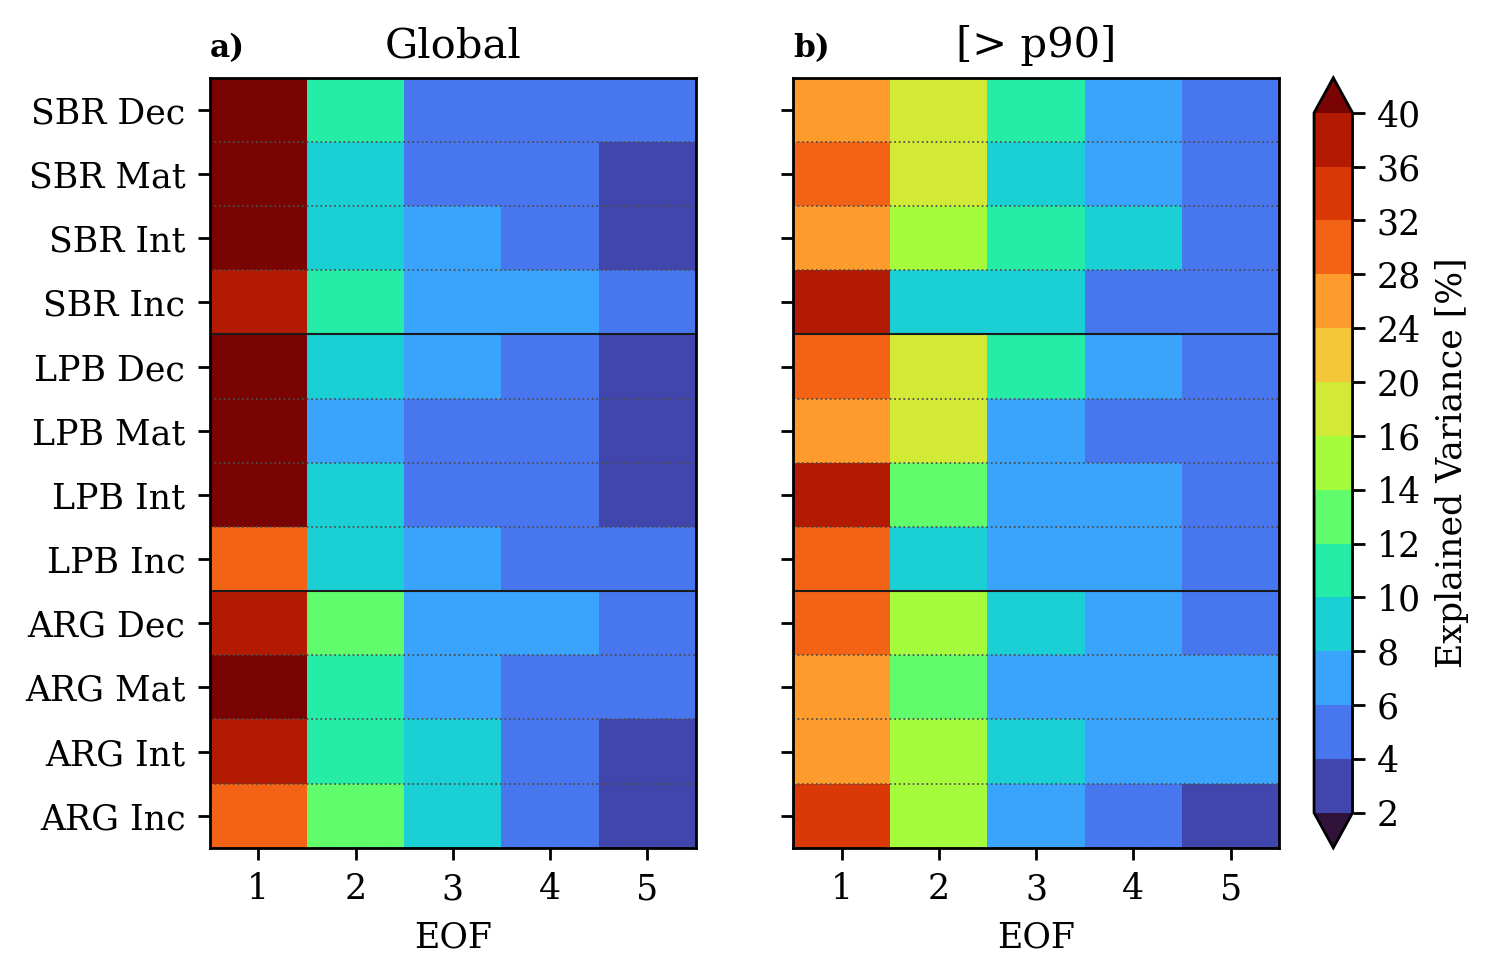
\includegraphics[width=0.8\textwidth]{images/w10/all_expvar_wind10_mean2times.png} 
\caption[Varianza explicada por los primeros cinco modos (EOF1--EOF5) de viento a 10~m]{Fraccionamiento de la varianza espacial total contenida en los primeros cinco modos dominantes (EOF1 a EOF5) del viento a 10~metros, obtenida mediante el procedimiento descrito en la Sección~\ref{subsec:eof_univariado}. Se contrasta la distribución de la varianza de la Población Global frente al subconjunto de intensidad p90 a lo largo del ciclo de vida para cada región de ciclogénesis.}
\label{fig:var_exp_wind10}
\end{figure}

La Figura~\ref{fig:var_exp_wind10} resume la varianza espacial distribuida en los primeros cinco modos ortogonales (EOF1 a EOF5) del campo de viento superficial, contrastando la Población Global (panel~a) frente al subconjunto p90 (panel~b) a lo largo de las fases evolutivas y para cada región de ciclogénesis.
En la Población Global, el modo EOF1 domina sobre los modos secundarios (EOF2 a EOF5) en todas las regiones y fases. 
Su concentración es máxima durante la fase de madurez, donde alcanza el 57.4\% en SBR y el 57.1\% en LPB, generando una
caída abrupta hacia los modos secundarios, que retienen porciones menores de varianza. 
ARG presenta valores algo menores entre 30.9\% y 43.3\%.
Este patrón refuerza la idea que la dinámica del viento superficial está gobernada por un único patrón espacial dominante en la Poblacion Global, coherente con un gradiente de gran escala como el flujo sinóptico de fondo.

En el subconjunto p90, la distribución de varianza cambia, el EOF1 no supera el 37.6\% en ninguna combinación de región y fase, con mínimos de hasta el 25.4\% durante la intensificación en ARG. 
Como consecuencia, la varianza se reparte entre múltiples modos, elevando la importancia relativa de EOF2 y EOF3 respecto a la Población Global. 
Este aplanamiento del espectro de autovalores es, de acuerdo con \citet{hannachi2007empirical}, el indicador de que la energía del sistema se ha distribuido entre modos competitivos de distinta escala espacial.
La divergencia entre ambas distribuciones responde a la complejidad estructural que adquieren los ciclones p90. 
Al profundizarse, el vórtice toma partido la no linearidad, repercutiendo en el frente, corrientes en chorro de bajos niveles y seclusiones térmicas (Sección~\ref{subsec:tb_modelos}). 
Estas estructuras de mesoescala compiten entre sí por la energía cinética del campo, de modo que la descomposición matemática requiere múltiples dimensiones ortogonales (EOF2--EOF5) para reconstruir la cinemática del ciclón, donde un único modo resulta insuficiente.

Estos resultados constituyen una demostración cuantitativa de que la severidad ciclónica no equivale a un escalado lineal de un sistema ordinario. 
La necesidad de múltiples modos para explicar los sistemas p90 implica que parametrizar vientos destructivos asumiendo los
patrones simples de la población media subestimará sistemáticamente tanto la agresividad como la naturaleza asimétrica y la localización de los máximos de viento.
%%%%%%%
\subsection{EOF1 --- Población Global}\label{subsec:eof1_wind10_global}

\begin{figure}[htbp]
\centering
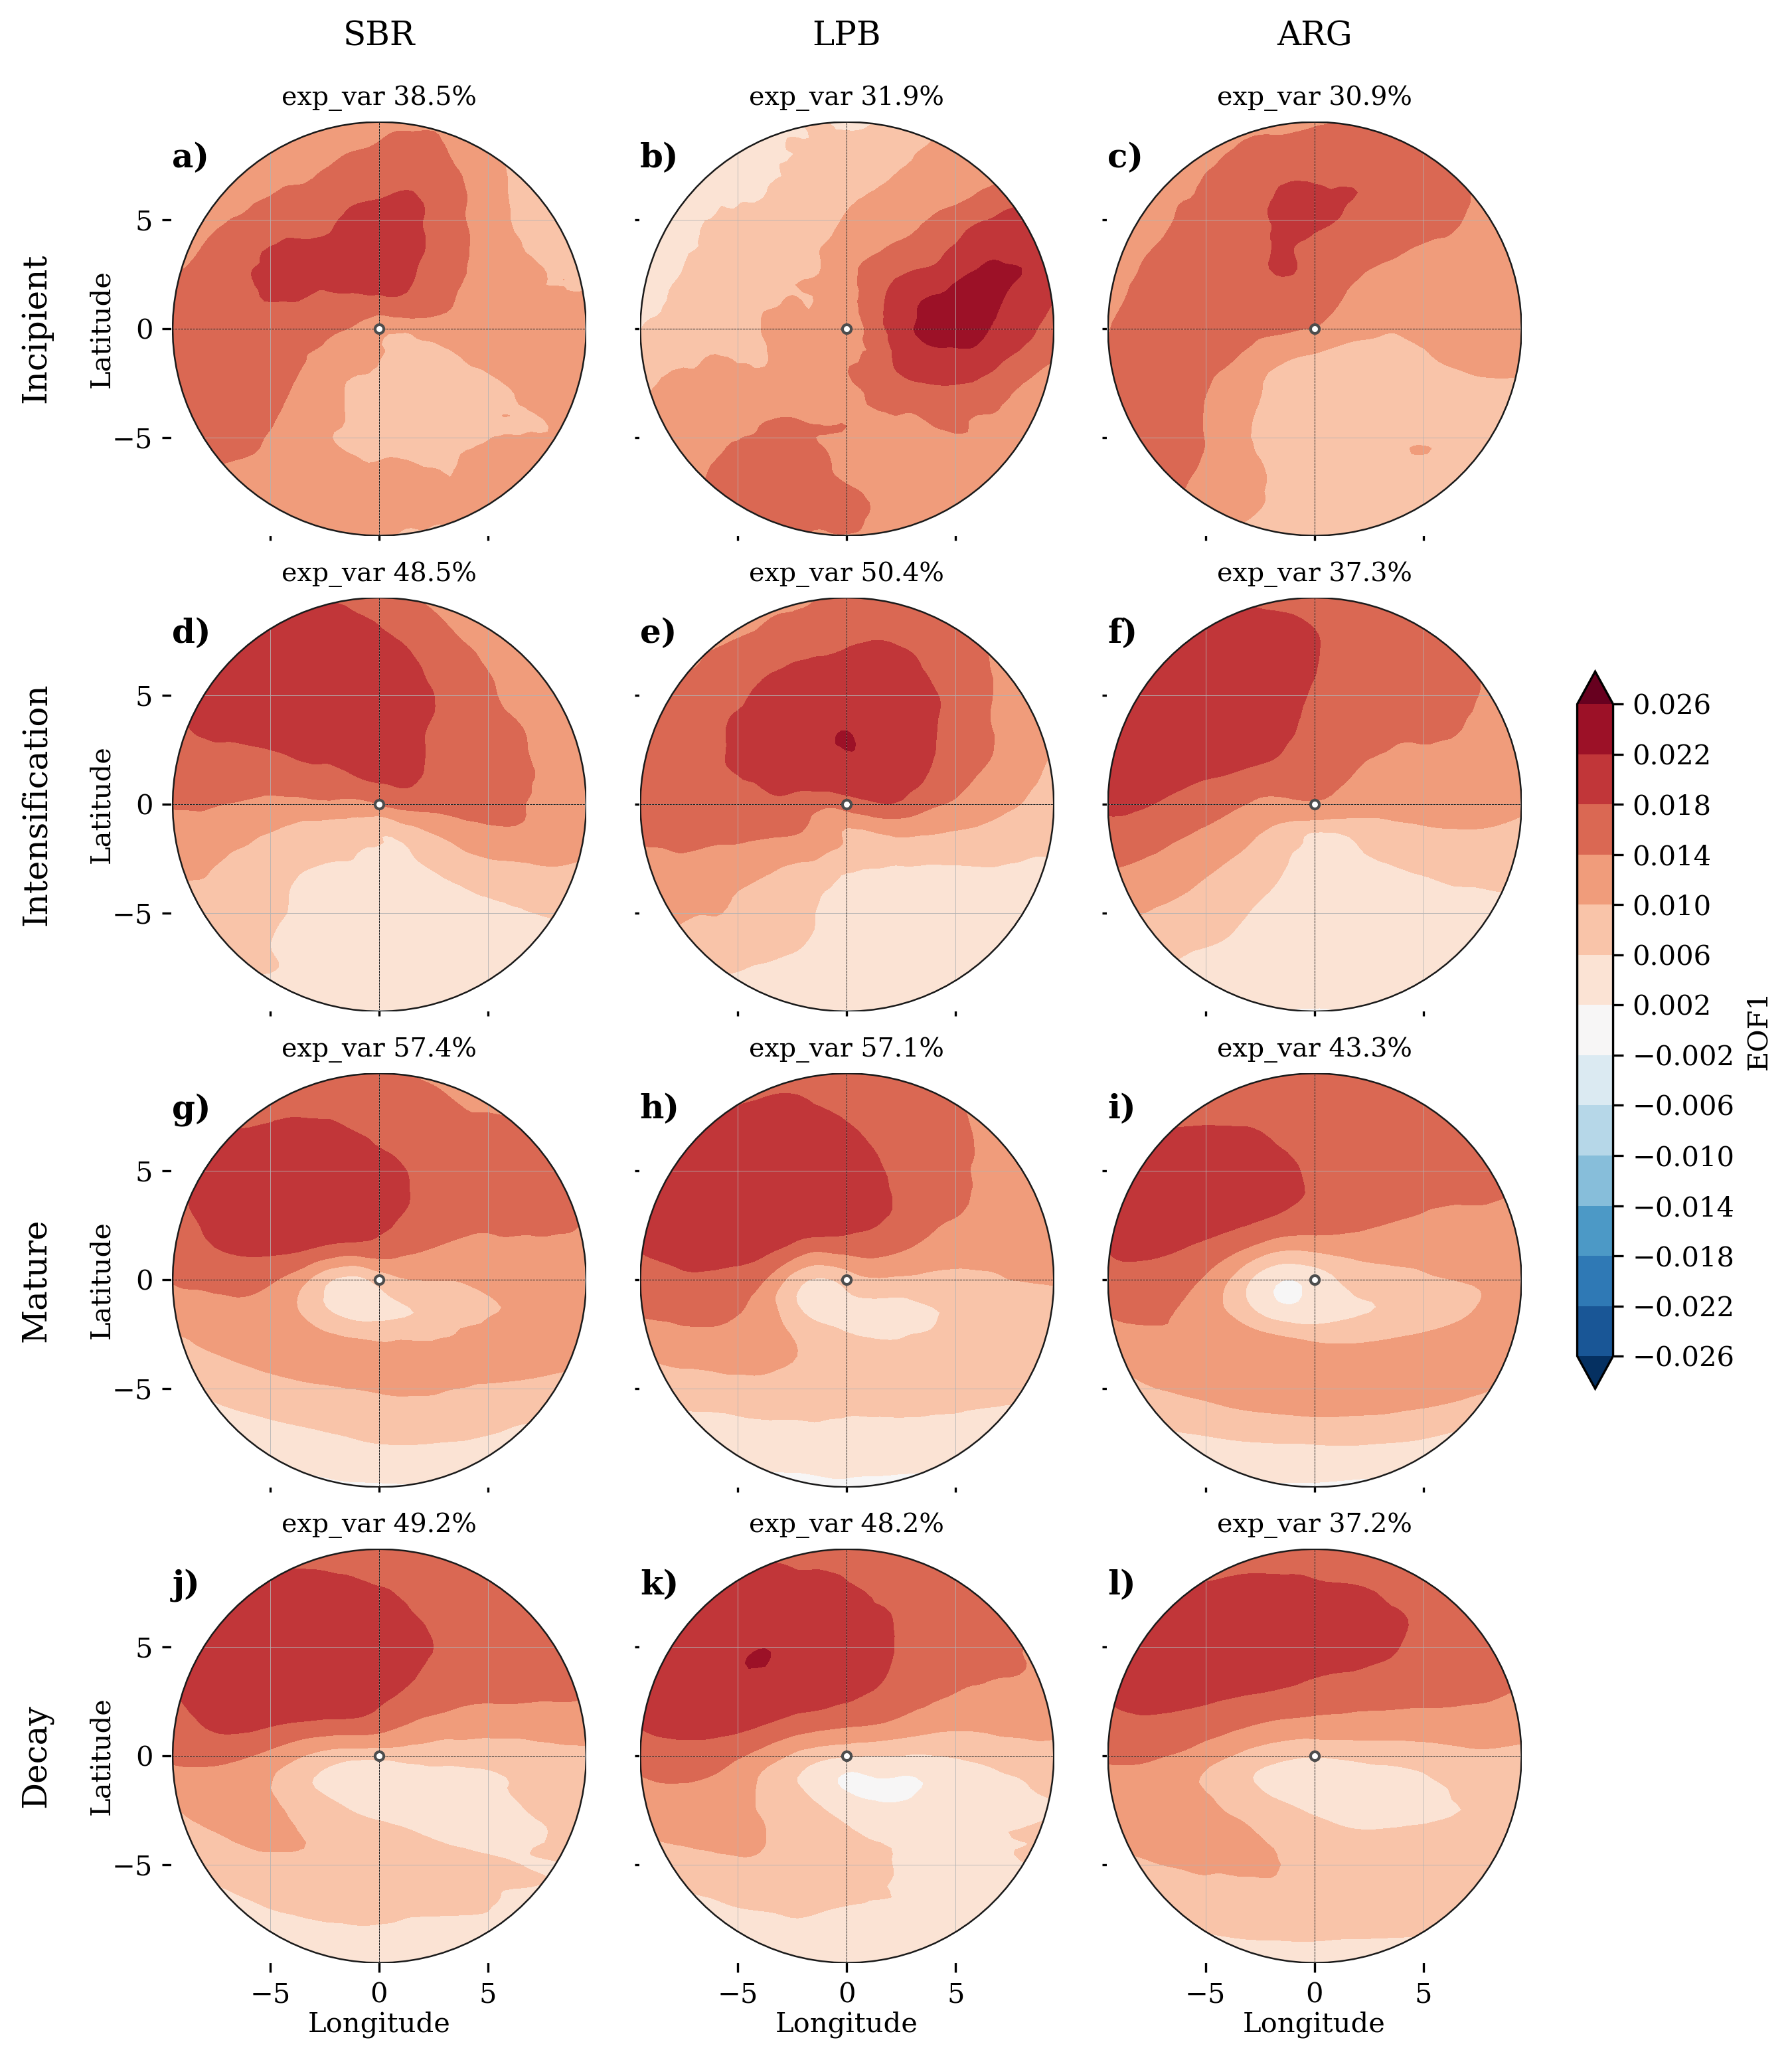
\includegraphics[width=\textwidth]{images/w10/pca1_wind10_global_fasesxreg.png}
\caption[EOF1 de la magnitud del viento a 10 metros --- Población Global]{Primer modo espacial (EOF1) de la magnitud del viento a 10~metros para la Población Global de referencia, derivado del análisis descrito en la Sección~\ref{subsec:eof_univariado}. Los paneles (a--c) corresponden a la fase incipiente (Ic) para las regiones SBR, LPB y ARG, respectivamente; (d--f) a la intensificación (It); (g--i) a la madurez (M); y (j--l) al decaimiento (D). El título de cada panel indica el porcentaje de varianza explicada (\textit{exp\_var}) por este modo dominante. Los colores cálidos (fríos) representan anomalías positivas (negativas) de la estructura del viento relativo al centro del ciclón en un dominio de $20^{\circ} \times 20^{\circ}$.}
\label{fig:eof1_wind10_global}
\end{figure}

La Figura~\ref{fig:eof1_wind10_global} presenta el primer modo de las Funciones Ortogonales Empíricas (EOF1) del campo de viento a 10~metros sobre el dominio lagrangiano. 
Tal como se evidenció en el fraccionamiento de energía (Sección~\ref{sec:var_exp_wind10}), el EOF1 domina ampliamente la varianza en la Población Global, con valores que oscilan entre el 30.9\% (ARG incipiente) y el 57.4\% (SBR madurez) según la región y fase evolutiva.
Morfológicamente, el patrón está organizado como un debil dipolo norte--sur de gran escala en el que las anomalías positivas dominan el sector norte del dominio (tonos rojos, $+0.010$ a $+0.026$), mientras que anomalías negativas o neutras se concentran en el sector sur y en las inmediaciones del centro ciclónico (tonos blancos--rosados tenues).
Este dipolo se consolida progresivamente desde la fase incipiente hasta la madurez, donde alcanza su mayor definición espacial y su varianza explicada más elevada en SBR (g, 57.4\%) y LPB (h, 57.1\%). 
La excepción es LPB en intensificación (e), donde el núcleo positivo se centraliza proximo al vórtice en lugar de desplazarse hacia el norte---noroeste, un patrón morfológicamente distinto al del resto regiones. 
En el decaimiento (j, k, l), las tres regiones se asemejan en la distribucion de la huella positiva al noroeste con un atenúamiento progresivo hacia el sector sureste; el dominio adopta una cobertura casi uniforme de anomalías positivas débiles.

La presencia de este el patron norte--sur desde intensificacion hasta la madurez, junto con su elevada varianza explicada, da indicios que la principal fuente de variabilidad en los ciclones está dictada por su interacción con el flujo zonal de fondo y las fluctuaciones del gradiente latitudinal de temperatura. 
% Como establece \citet{hannachi2007empirical} y se fundamenta en la Sección~\ref{subsubsec:tb_eof}, la emergencia de una estructura dipolar en EOF1  constituye la firma matemática del desplazamiento posicional de una corriente de gran escala; en el Hemisferio Sur, esto se traduce en oscilaciones de la latitud relativa de las corrientes en chorro en la alta troposfera. 
De acuerdo con \citet{hoskins2005new} y \citet{dossantos2023response}, la evolución estructural de los ciclones depende del acoplamiento baroclínico, de modo que las anomalías capturadas por EOF1 reflejan cómo el sistema expande o contrae su campo de viento en respuesta a la posición del chorro, expansión que \citet{simmonds2000size} documentan como un aumento sistemático del radio ciclónico durante el desarrollo.
La excepción geométrica de LPB en intensificación (e) respalda la dependencia de los forzantes físicos locales. 
De acuerdo con \citet{gramcianinov2019properties}, los sistemas en esta zona están modulados en sus etapas iniciales por la influencia de la baja orográfica, lo que ancla la varianza del viento a forzantes topográficos centralizados y retrasa temporalmente la imposición de un debil dipolo zonal de gran escala característico de las demás regiones y fases.

En el decaimiento, al debilitarse progresivamente el sistema, la circulación ciclónica pierde definición y la variabilidad de su componente cinemática queda supeditada a los desplazamientos del gradiente de presión meridional del entorno. 
La perturbación queda inmersa en el flujo de mayor escala, lo que concuerda con la zonificación descrita por \citet{inatsu2004zonal}, quienes documentan que las trayectorias invernales del Hemisferio Sur presentan una asimetría zonal organizada por el flujo estacionario de latitudes medias, modulando la disipación de los sistemas sinópticos.
Este patrón univariado establece la línea base de variabilidad estructural del ciclón extratropical, necesaria para la comparación posterior con los eventos intensos y con el análisis multivariado (Sección~\ref{sec:meof_prototipos}).
%%%%%%
\subsection{EOF1 --- Subconjunto p90}\label{subsec:eof1_wind10_p90}

\begin{figure}[htbp]
\centering
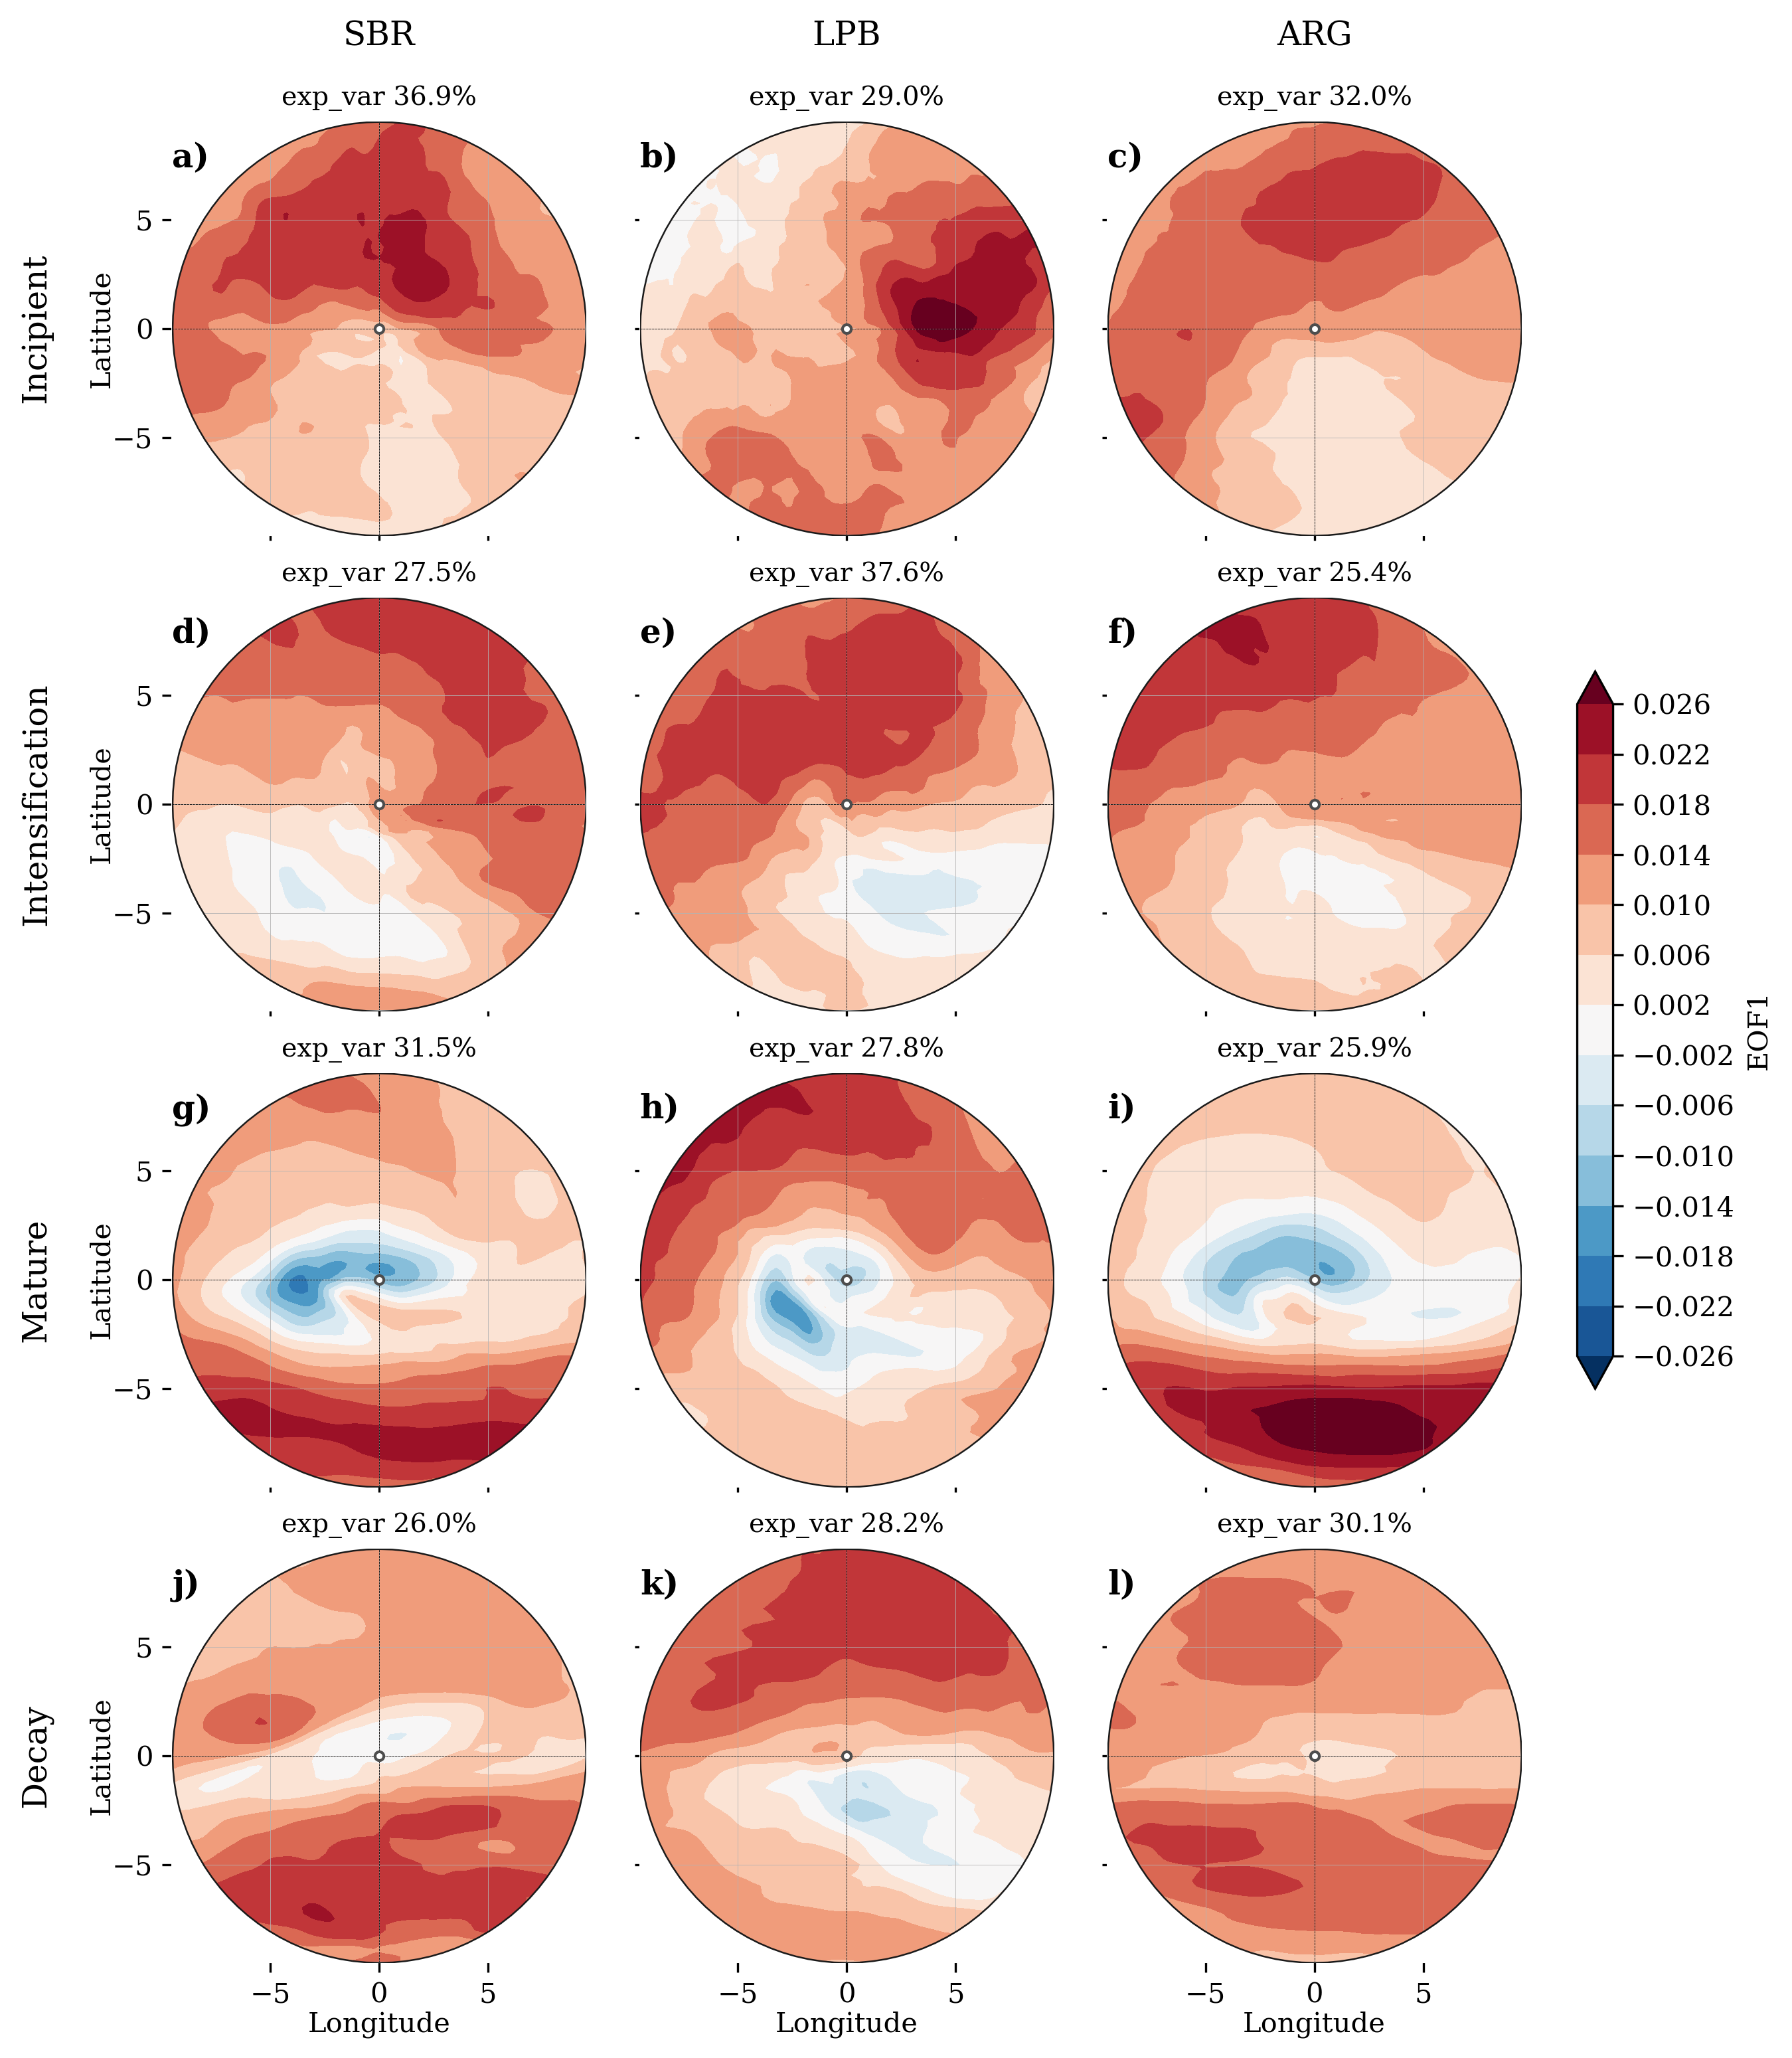
\includegraphics[width=\textwidth]{images/w10/pca1_wind10_p90_fasesxreg.png}
\caption[EOF1 de la magnitud del viento a 10 metros --- Subconjunto p90]{Primer modo espacial (EOF1) de la magnitud del viento a 10~metros para el subconjunto de ciclones intensos (p90). La disposición de los paneles (a--l) por región de ciclogénesis (columnas) y fase evolutiva (filas) es idéntica a la
Figura~\ref{fig:eof1_wind10_global}. Se detalla la varianza explicada (\textit{exp\_var}) en cada panel y la barra de color estandarizada para evaluar
las diferencias en las firmas espaciales de los eventos intensos frente al comportamiento climatológico.}
\label{fig:eof1_wind10_p90}
\end{figure}

El contraste contra la Población Global revela que los ciclones p90 no amplifican el patrón base sino que reconfiguran su estructura modal. 
En p90, la varianza capturada por EOF1 se reduce respecto a la Población Global, oscilando entre el 25.4\% y el 37.6\%, y el patron muestra firmas más complejas e hiperlocalizadas que el dipolo debil norte--sur de gran escala observado en la Sección~\ref{subsec:eof1_wind10_global}.

La evolución morfológica por fases evidencia esta reconfiguración. 
En la fase incipiente (a, b, c), las tres regiones muestran patrones difusos con anomalías positivas que dominan el sector norte y noreste, sin una estructura dipolar bien definida, coherente con la baja organización esperada en esta etapa. 
Durante la intensificación (d, e, f), emerge un dipolo norte--sur más definido, las anomalías positivas se concentran en el norte, noreste y noroeste mientras que anomalías negativas débiles aparecen en el sector sur en general, con ARG (f) mostrando la señal más intensa ($>+0.022$ en el noroeste). 
El mayor cambio ocurre en la madurez (g, h, i): las tres regiones desarrollan un dipolo asimétrico con un núcleo negativo compacto e intenso localizado alrededor y al oeste del centro ciclónico, rodeado por anomalías positivas que dominan el norte y el sur del dominio. 
Este núcleo negativo es particularmente intenso en LPB (h) y ARG (i), mientras que en SBR (g) las anomalías negativas se extienden hacia el suroeste con valores que alcanzan $-0.022$. 
En el decaimiento (j, k, l), el dipolo pierde definición y el dominio retorna a una cobertura predominantemente positiva con gradientes más suaves, aunque los contornos negativos se aproxima al núcleo en SBR y LPB.

La hiperlocalización de las anomalías en la madurez son la manifestación espacial de la fragmentación de energía multiescalar discutida en la Sección~\ref{sec:var_exp_wind10}. 
En estos eventos, la intensa circulación cerrada de mesoescala domina sobre el flujo de fondo, de modo que el EOF1 ya no captura un gradiente sinóptico de gran escala sino la variabilidad en la posición e intensidad de estructuras mesoescalares internas. 
De acuerdo con la localización espacial discutida en la Sección~\ref{sec:kde_espacial_p90}, la cinta transportadora fría (CCB) y los procesos de fractura frontal se traducen en un EOF1 compacto e hiperlocalizado, cuya estructura no puede representarse mediante un patrón de gran escala.

El patrón de ARG en madurez (i) merece una lectura diferenciada. 
La combinación de anomalías negativas intensas en el centro---norte y positivas en el sur configura una firma que indica fluctuaciones en el tamaño de la seclusión cálida (\textit{warm seclusion}; Secciones~\ref{subsec:tb_modelos} y~\ref{subsec:tb_fases}).
Como detallan \citet{schultz2021antecedents}, \citet{reboita2022from} y \citet{shapiro1999bridge}, la formación de esta seclusión en el núcleo rodeada por un anillo de vientos es el rasgo evolutivo del modelo conceptual de \citet{shapiro1990life}, una vía de desarrollo característica de ciclones con alta organización baroclínica.

En conjunto, estos resultados demuestran que un ciclón intenso no es estructuralmente equivalente a un ciclón ordinario, su dinámica modifica la morfologia modal del campo de viento. 
Esta separación morfológica concuerda con el espacio de fases de \citet{hart2003cyclone}, que demuestra que las fluctuaciones en la asimetría térmica y
el espesor de capa definen caminos evolutivos distintivos. 
Como enfatizan \citet{corner2025classification} y \citet{eisenstein2023identification}, la intensidad del viento superficial no depende únicamente de la sinóptica de gran escala, sino de la manifestación explícita de estas estructuras mesoescalares internas.
%%%%%%%%
\subsection{Significancia estadística}\label{subsec:res_significancia_madurez}

Para discriminar entre señales físicas y fluctuaciones estocásticas propias del remuestreo, se evaluó la significancia estadística de los autovectores espaciales mediante el método Bootstrap-tt, cuyos fundamentos se describen en la Sección~\ref{subsec:bootstrap_significancia} siguiendo a \citet{hesterberg2015bootstrap}.
La Figura~\ref{fig:xeof_madurez_global} documenta los tres primeros modos (EOF1--EOF3) y sus series temporales (PC1--PC3) para la Población Global en fase de madurez, mientras que la Figura~\ref{fig:xeof_madurez_p90} presenta el análisis equivalente para el subconjunto p90. 
El achurado delimita las áreas estadísticamente significativas al 95\% de confianza.

\begin{figure}[htbp]
\centering
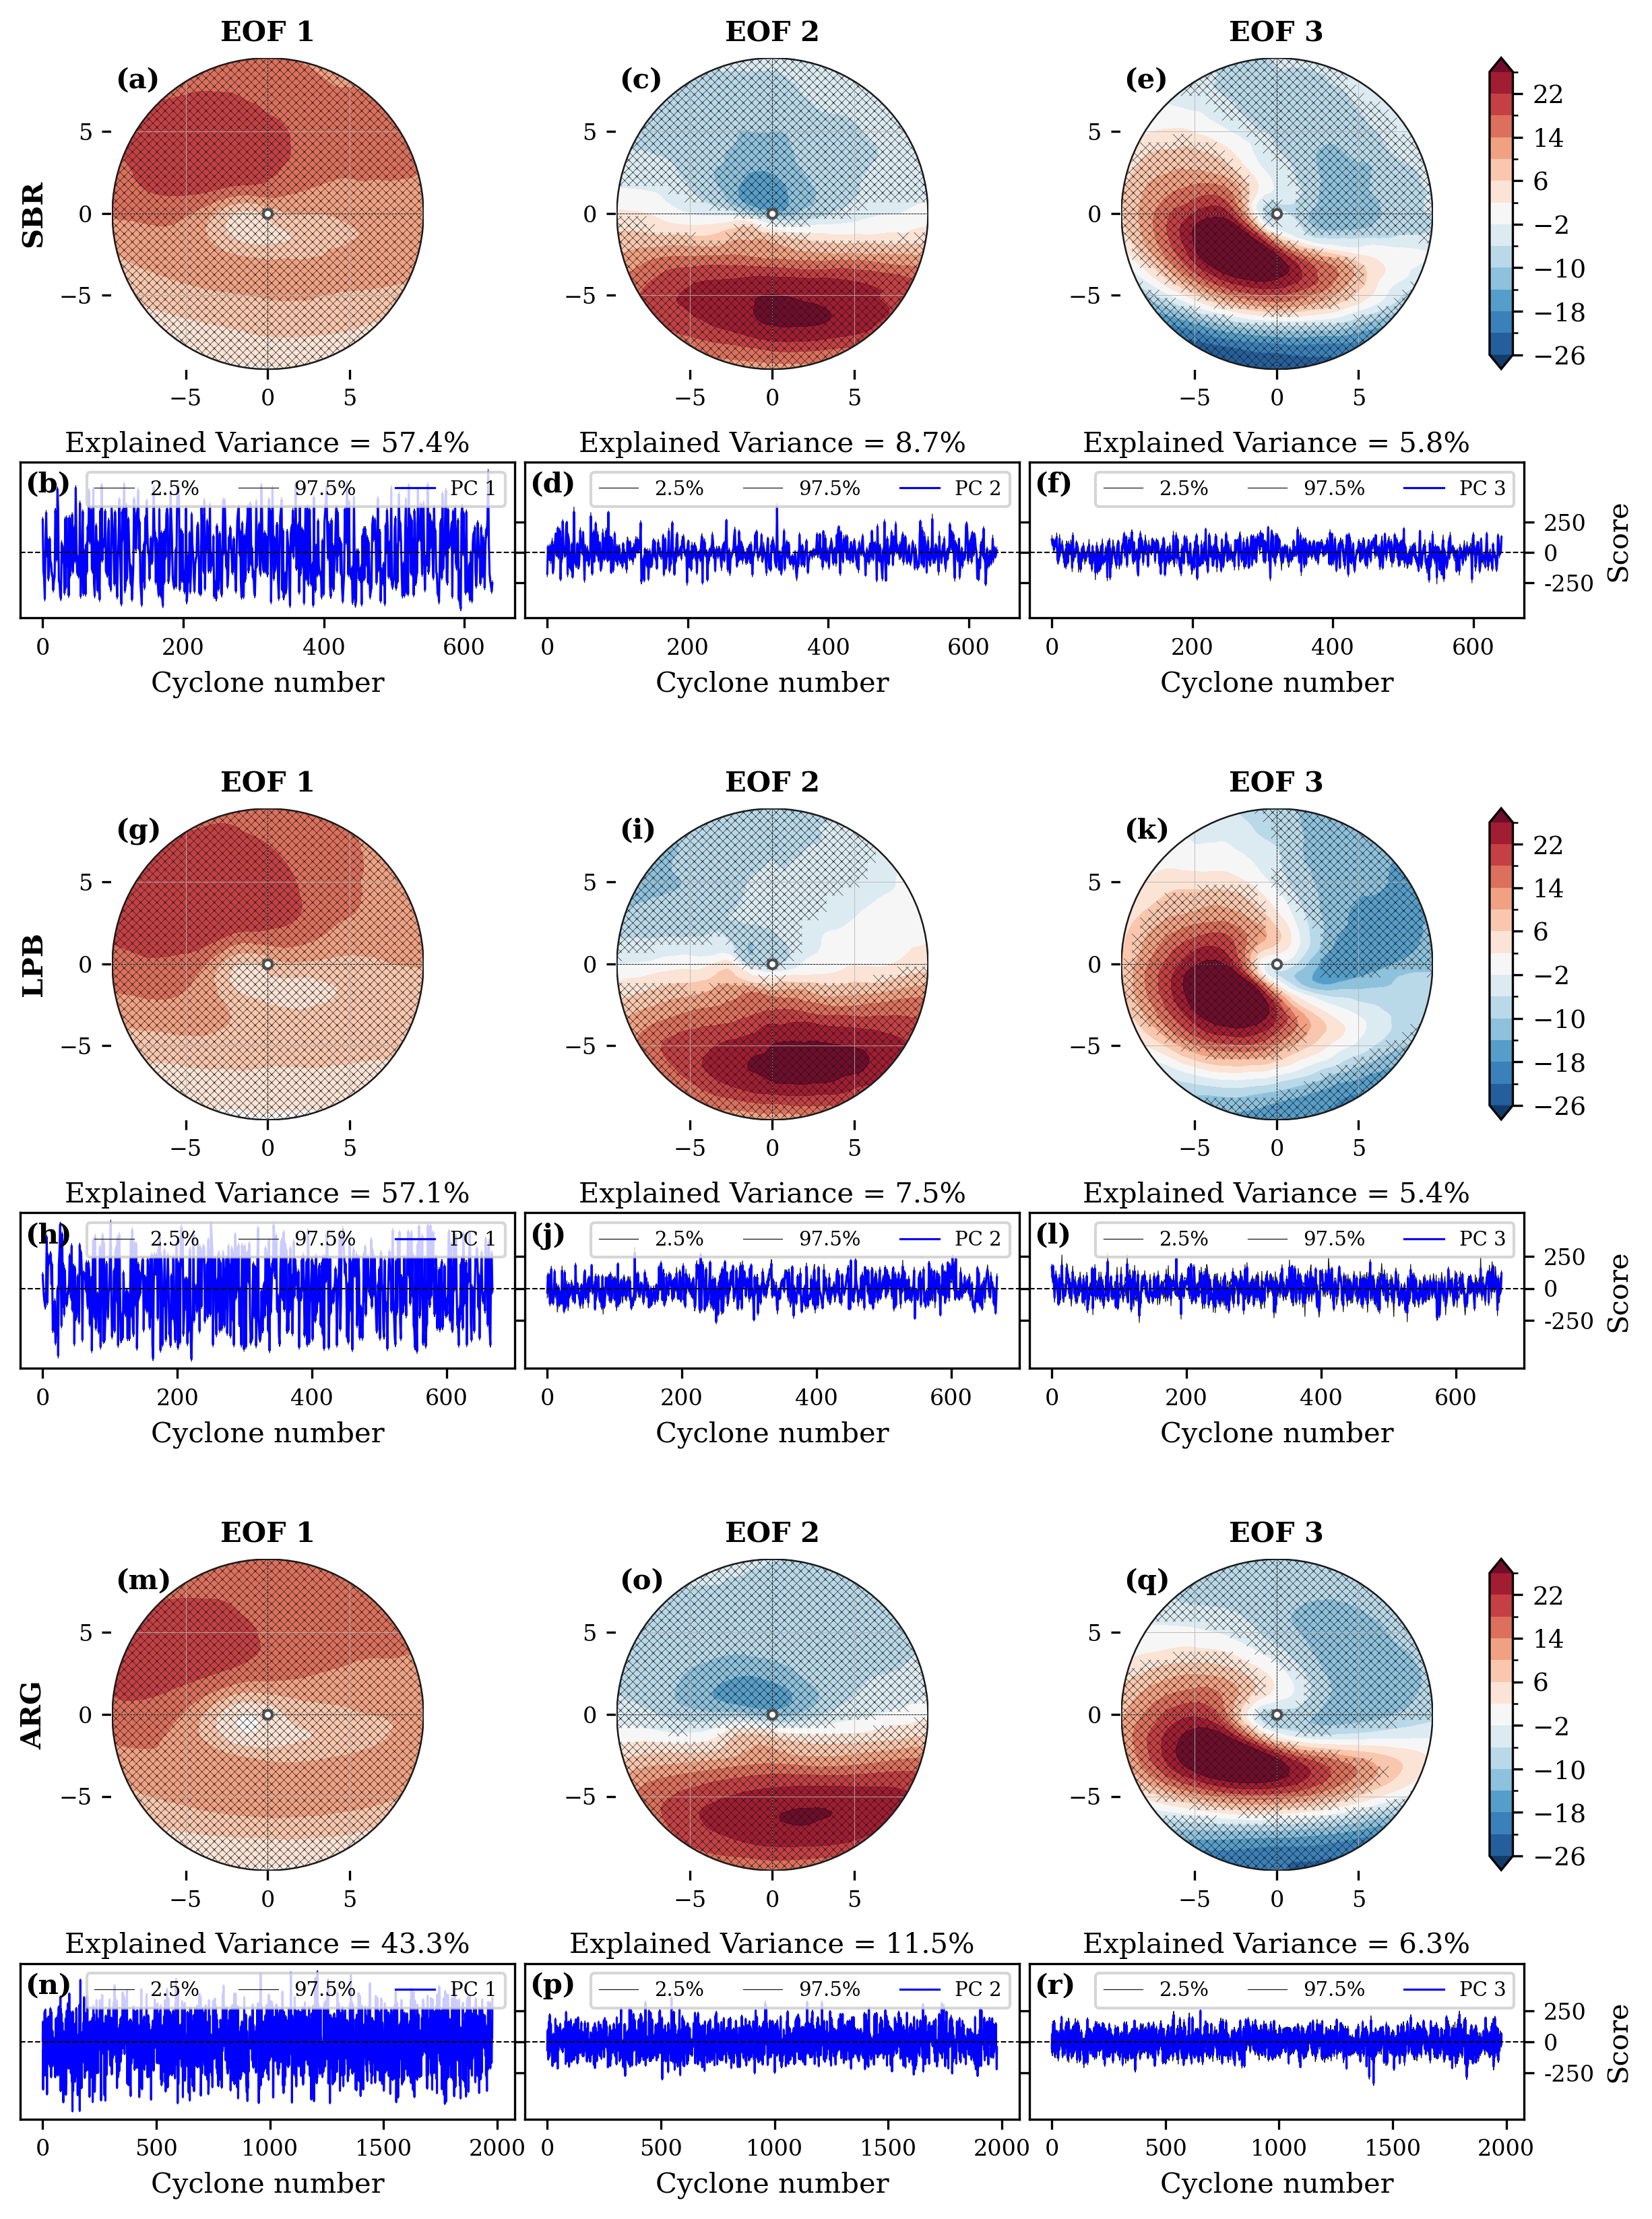
\includegraphics[width=\textwidth]{images/w10/xeof_global_wind10_mature.png}
\caption[Significancia espacial de los EOFs en fase de madurez --- Población Global]{Descomposición EOF del viento a 10~m para la Población Global en fase de madurez. Paneles (a, g, m): mapas de EOF1 para SBR, LPB y ARG respectivamente; (c, i, o): EOF2; (e, k, q): EOF3. El achurado indica significancia estadística al 95\% (test Bootstrap-tt; Sección~\ref{subsec:bootstrap_significancia}). Paneles (b, h, n): series temporales de PC1; (d, j, p): PC2; (f, l, r): PC3. La línea gris delimita los percentiles 2.5 y 97.5 de la distribución bootstrap.}
\label{fig:xeof_madurez_global}
\end{figure}

\begin{figure}[htbp]
\centering
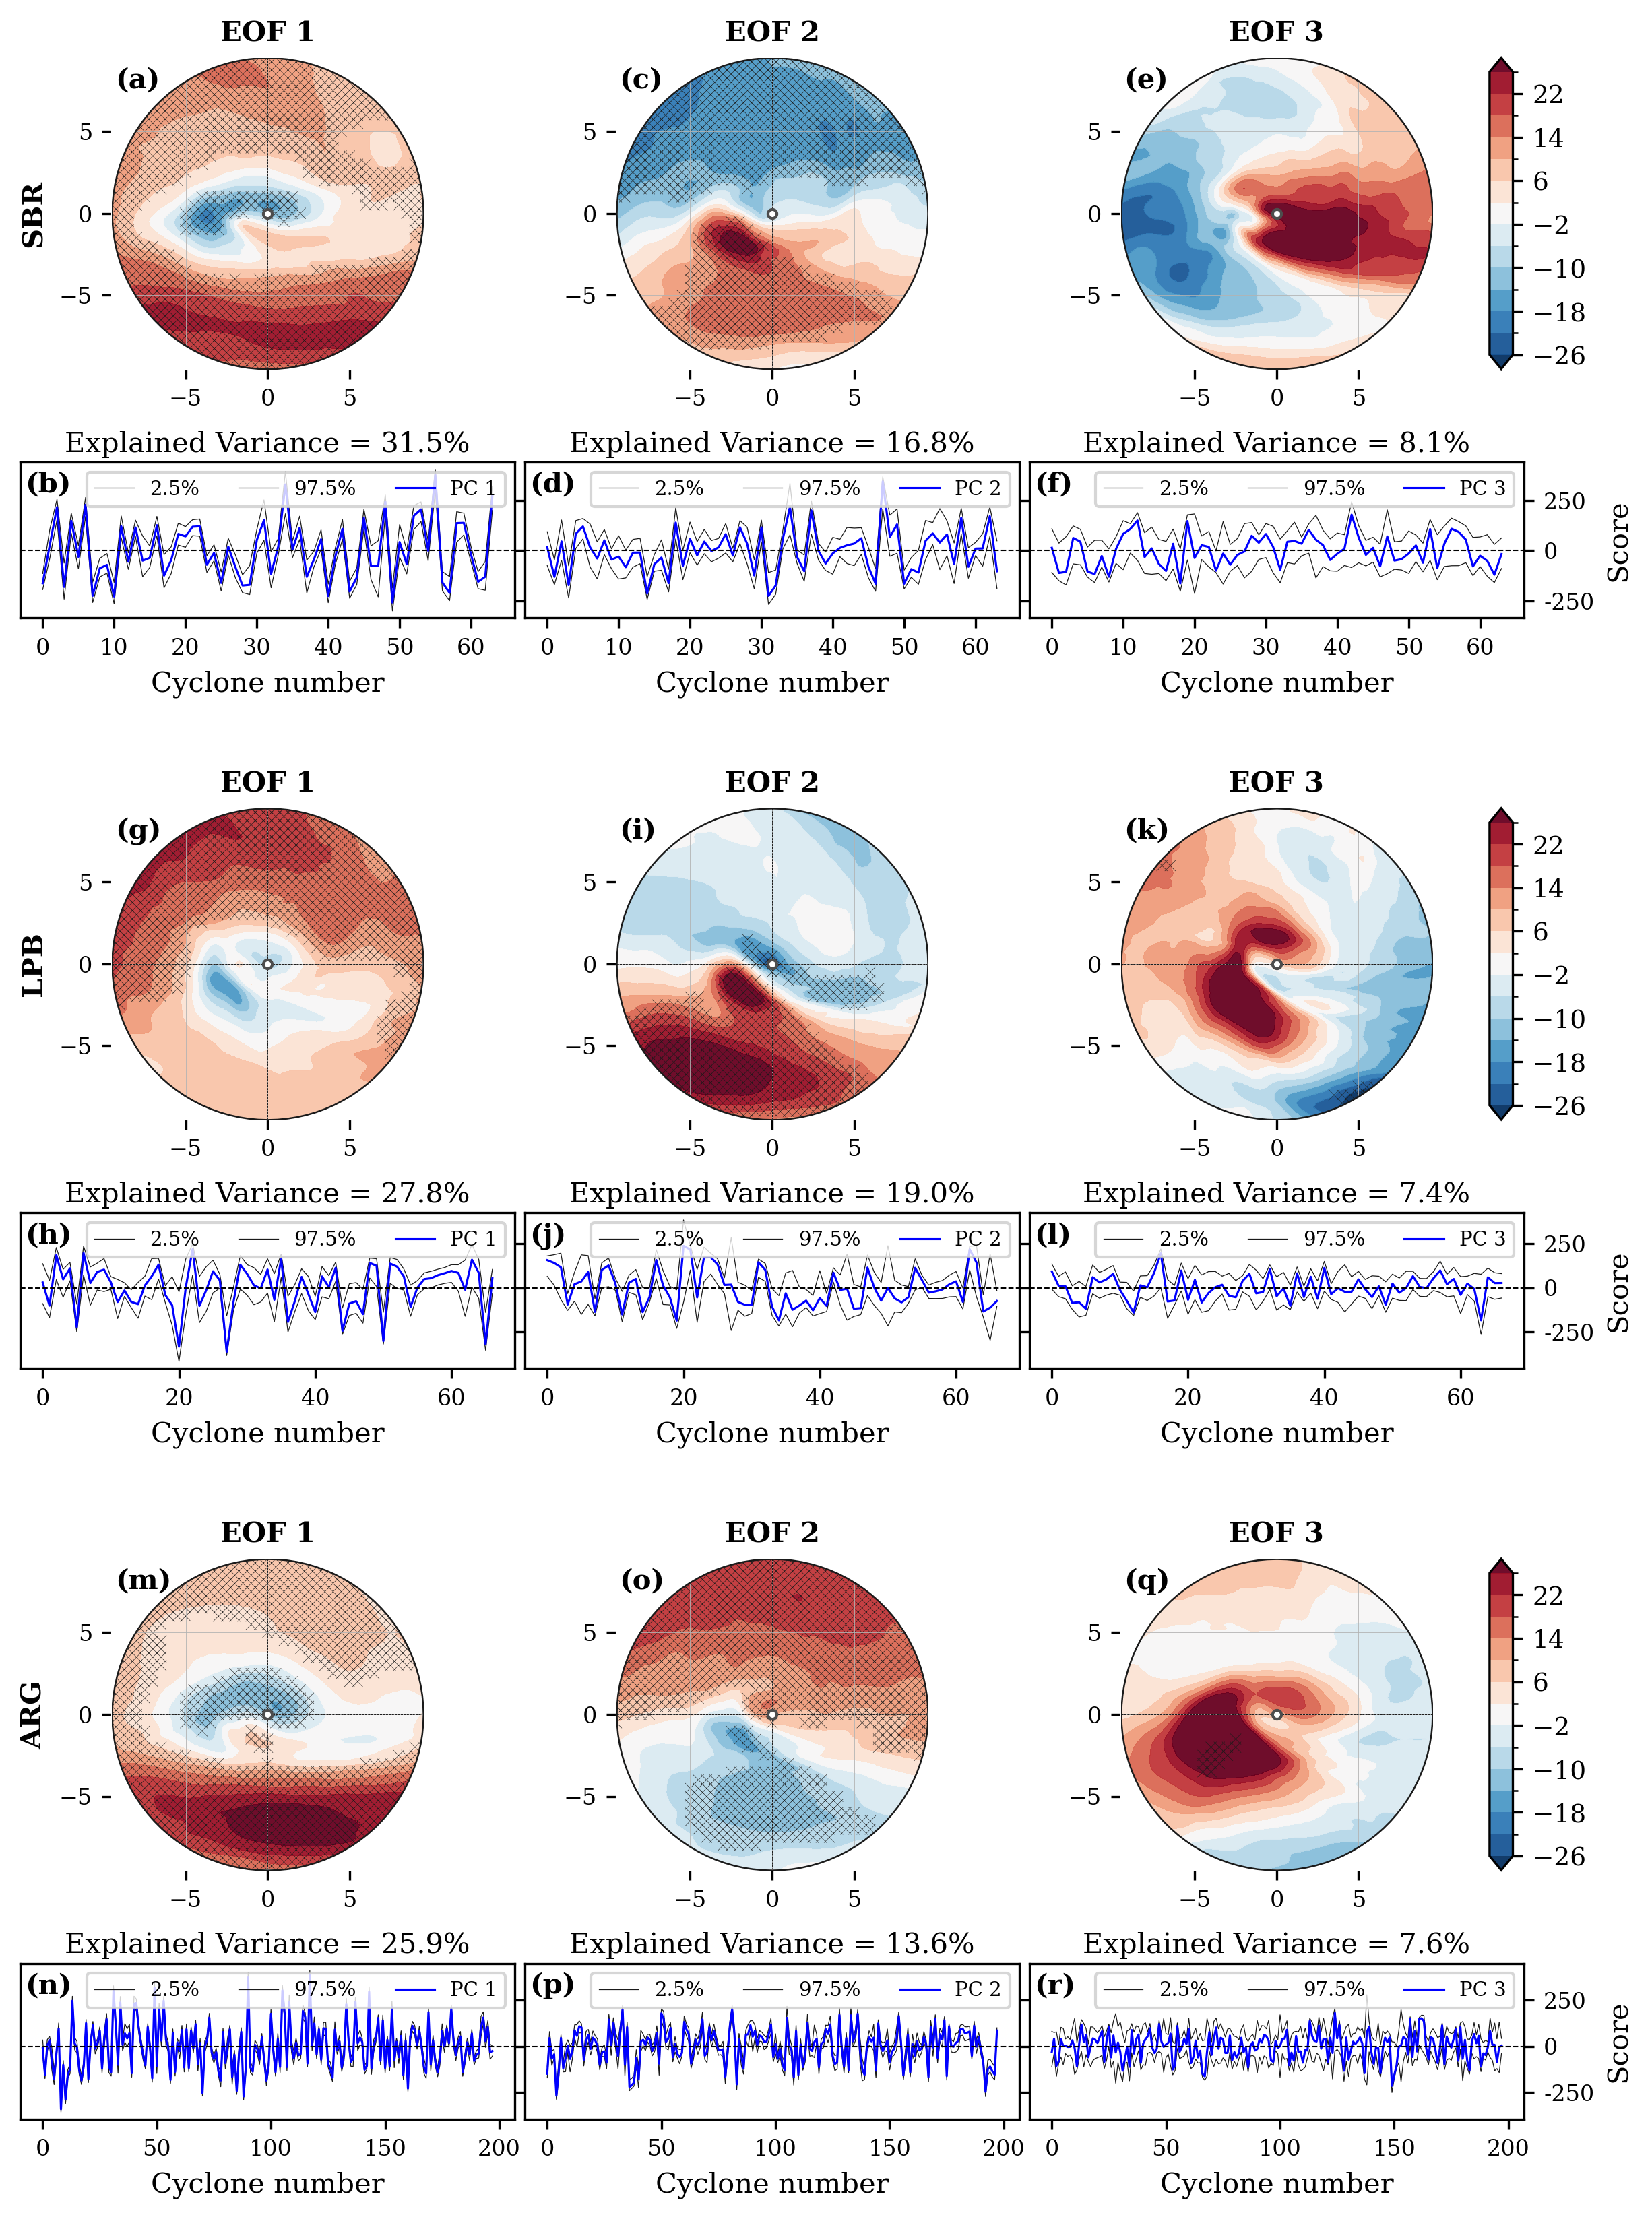
\includegraphics[width=\textwidth]{images/w10/xeof_p90_wind10_mature.png}
\caption[Significancia espacial de los EOFs en fase de madurez --- Subconjunto p90]{Descomposición EOF del viento a 10~m para el subconjunto intenso (p90) en fase de madurez. La disposición de paneles es idéntica a la Figura~\ref{fig:xeof_madurez_global}.}
\label{fig:xeof_madurez_p90}
\end{figure}

En la Población Global (Figura~\ref{fig:xeof_madurez_global}), el EOF1 exhibe áreas de significancia que abarcan el dominio en total del sistema ciclónico en las tres regiones (paneles a, g, m para SBR, LPB y ARG, respectivamente).
Esta respuesta de patrón dominante puede asociarse al incremento de la conversión barotrópica de energía durante la madurez documentada por \citet{coutodesouza2024thesis} en ciclones extratropicales, entendiendo así que el patrón constituye una característica física estable de los sistemas en su fase madura.
Consistente con la alta varianza explicada (43--57\%), las series de PC1 (paneles b, h, n) presentan amplitudes mayores que las de los modos secundarios. Entre regiones, SBR y LPB muestran fluctuaciones de amplitud comparable en PC1, mientras que ARG exhibe una dispersión ligeramente mayor y más irregular.

Los modos EOF2 y EOF3 de la Población Global exhiben estructuras significativas confinadas a sectores específicos del dominio. En EOF2 se presenta la transición latitudinal respecto al centro, variando de en patron positivo a negativo en las tres regiones, mientras que en EOF3 se tiene el gradiente zonal. 
La interpretación de \citet{hannachi2007empirical}, quienes establecen que el EOF2 captura estructuras ortogonales al modo dominante, representando en este caso las fluctuaciones de circulación de mesoescala y asimetría secundaria del campo de viento.
En términos regionales, SBR y ARG presentan estructuras significativas de EOF2 más extendidas (paneles c y o) en comparación con LPB (panel i), donde no es significantiva en el cuadrante noreste.
Esta diferencia espacial se refleja en las series temporales: las PC2 de SBR (panel d) muestran episodios de alta amplitud más frecuentes que en LPB (panel j), indicando una mayor variabilidad de mesoescala en SBR.

Las PC3 mantienen amplitudes comparativamente atenuadas en las tres regiones (paneles f, l, r), consistente con su menor varianza explicada (5,4--6,3\%).
Dado que en la Población Global la separación entre autovalores es pronunciada, los modos secundarios describen variabilidad residual de menor magnitud física. 
Sin embargo, la comparación entre regiones revela que SBR concentra mayor variabilidad explicada por EOF2 (8,7\%) que LPB (7,5\%) y que ARG (11,5\%), lo cual sugiere que los sistemas en ARG experimentan procesos de mayor complejidad dinámica durante la madurez.
En contraste, la estructura de EOF3 resulta notablemente similar entre regiones (5,4--6,3\%), indicando que los gradientes zonales de viento constituyen un mecanismo general de variabilidad residual en la fase madura.

En el subconjunto p90 (Figura~\ref{fig:xeof_madurez_p90}), el patrón de significancia se transforma cualitativamente.
El EOF1 presenta una contracción variable entre regiones; en SBR (panel a) y ARG (panel m), la significancia se concentra en las áreas de anomalía positiva (sur y sureste, respectivamente), mientras que sobre el núcleo negativo (nor-noroeste en SBR, noroeste en ARG) la significancia es más limitada, aunque no completamente ausente. 
En LPB (panel g), la significancia de este patron permanece extenso en la región positiva del norte, noroeste y también cubre parcialmente el cuadrante noreste, excepto al rededor del centro, donde se tienen anomalias negativas aunque no son significtivas.
Esta reducción de significancia sobre zonas específicas indica que el EOF1 captura preferentemente la envolvente sinóptica de gran escala, pero no logra representar de manera estadísticamente robusta algunas estructuras mesoescalares localizadas que caracterizan a los ciclones intensos.

El contraste más relevante del subconjunto p90 reside en el comportamiento de EOF2 y EOF3. 
A diferencia de la Población Global donde estos modos son residuales, en p90 los patrones EOF2 (paneles c, i, o) y EOF3 (paneles e, k, q) presentan áreas de significancia estadística que en varios casos superan en extensión ala del propio EOF1.
Morfológicamente, EOF2 exhibe estructuras compactas e hiperlocalizadas alrededor del núcleo ciclónico en las tres regiones, este patron se puede relacionar a la posición e intensidad del jet de la cinta transportadora fría (CCB, \textit{cold conveyor belt}).
El chorro de bajo nivel que se forma en la cola del frente doblado (\textit{bent-back front}) responde al mismo mecanismo de intensificación por vorticidad potencial descrito para la CCB (Sección~\ref{sec:pdf_wind10}) \citep{schemm2014linkage}.

El comportamiento de las series temporales refuerza este diagnóstico. 
En la Población Global, PC2 y PC3 (paneles d, f para SBR; j, l para LPB; p, r para ARG) presentan amplitudes menores a los límites de la PC1.
En p90, en cambio, las amplitudes de PC2 (paneles d, j, p) y PC3 (paneles f, l, r) presentan magnitudes frecuentemente comparables a las de PC1 (paneles b, h, n). 
Los modos secundarios de p90 han dejado de ser ruido estadístico \citep{hannachi2023eof}, consistente con el aplanamiento del espectro de autovalores ya discutido (Sección~\ref{sec:var_exp_wind10}).

La competencia energética entre PC1, PC2 y PC3 en p90 es la expresión estadística de la fragmentación dinámica del campo de viento documentada en la Sección~\ref{sec:var_exp_wind10}; la CCB, los frentes y las seclusiones térmicas compiten simultáneamente por la energía cinética del sistema, obligando a la descomposición a distribuir la varianza entre múltiples dimensiones ortogonales en el sistema.
En conjunto, estos resultados cuantifican la reducción de predictibilidad espacial asociada a la intensidad ciclónica. 
En la población global, el patrón dipolar debil estadísticamente robusto del EOF1 permite caracterizar la distribución del campo de viento mediante un único modo dominante.
En p90, la señal del EOF1 se restringe a la sinóptica de gran escala, mientras que el núcleo mesoescalar ---donde se concentran los vientos más extremos--- queda capturado por EOF2 y EOF3, cuya significancia estadística (EOF2) en p90 constituye evidencia de que estas estructuras son físicamente recurrentes. 

\section{Componentes principales (PC1)}\label{subsec:res_dinamica_pc1}

La fragmentación de la varianza y la contracción de las áreas significativas observadas en la fase de madurez (Sección~\ref{subsec:res_significancia_madurez}) tienen su contraparte en el comportamiento de las Componentes Principales. 
Mientras que en la Población Global la PC1 domina la evolución del sistema ---evidenciado por sus amplitudes superiores y áreas significativas extensas---, en los ciclones p90 la competencia entre múltiples modos ortogonales (Figura~\ref{fig:xeof_madurez_p90}) se traduce en propiedades estadísticas distintivas, una correlación débil con el forzante sinóptico.

\begin{table}[htbp]
\centering
\caption[Momentos estadísticos y correlación de PC1--PC3 del viento a 10 m - Población Global]
{Asimetría ($\gamma_1$) y curtosis ($\gamma_2$) de la PC1 del viento a 10 metros, y correlación de Spearman ($r$) entre PC1, PC2 y PC3 (con signo) y la vorticidad relativa a 850 hPa asociada a la fase (con signo, negativa en el Hemisferio Sur), para la Población Global. El signo de la correlación depende de la convención de signo de cada EOF (Sección~\ref{subsec:analisis_pc}); lo relevante es que el lado del patrón dominante en que cae cada ciclón está asociado a su intensidad. Los valores significativos ($p<0.05$) se muestran en negrita.}
\label{tab:stat_global_w10}
\begin{tabular*}{\textwidth}{@{\extracolsep{\fill}}llrrrrr}
\hline
\textbf{Región} & \textbf{Fase} & \textbf{Asimetría ($\gamma_1$)} & \textbf{Curtosis ($\gamma_2$)} & \textbf{PC1} & \textbf{PC2} & \textbf{PC3} \\
\hline
\textbf{SBR} & Incipiente       & 0.58  & -0.12 & \textbf{-0.57} & \textbf{0.20} & \textbf{-0.37} \\
             & Intensificación & 0.26  & -0.91 & \textbf{-0.80} & 0.02 & \textbf{-0.32} \\
             & Madurez         & 0.30  & -0.86 & \textbf{-0.89} & 0.04 & \textbf{-0.25} \\
             & Decaimiento     & 0.24  & -0.79 & \textbf{-0.83} & \textbf{0.12} & \textbf{0.13} \\
\hline
\textbf{LPB} & Incipiente       & 0.99  & 1.32  & \textbf{-0.35} & \textbf{0.14} & \textbf{0.16} \\
             & Intensificación & 0.17  & -1.03 & \textbf{-0.71} & \textbf{-0.18} & \textbf{-0.12} \\
             & Madurez         & -0.09 & -1.01 & \textbf{-0.87} & \textbf{-0.09} & \textbf{-0.19} \\
             & Decaimiento     & -0.11 & -0.77 & \textbf{-0.83} & \textbf{-0.11} & \textbf{-0.09} \\
\hline
\textbf{ARG} & Incipiente       & 0.31  & -0.13 & \textbf{-0.43} & \textbf{0.24} & \textbf{0.06} \\
             & Intensificación & -0.22 & -0.37 & \textbf{-0.67} & \textbf{0.11} & \textbf{0.05} \\
             & Madurez         & -0.12 & -0.43 & \textbf{-0.86} & \textbf{0.05} & \textbf{-0.26} \\
             & Decaimiento     & -0.06 & -0.30 & \textbf{-0.76} & -0.04 & \textbf{-0.28} \\
\hline
\end{tabular*}
\end{table}


\subsection{Población Global: Patrón sinóptico dominante}

La Tabla~\ref{tab:stat_global_w10} documenta las métricas estadísticas (asimetría, curtosis) y la correlación de Spearman de la PC1 con la vorticidad mínima a 850~hPa para la Población Global, calculadas mediante el procedimiento descrito en la Sección~\ref{subsec:analisis_pc}. 

Al evaluar la evolución de la población global, la distribución de la PC1 exhibe una progresiva normalización estructural. 
En las tres regiones (SBR, LPB y ARG), los valores de curtosis oscilan de forma consistente entre $-0.30$ y $-1.03$ durante la intensificación y madurez, evidenciando distribuciones platicúrticas sin colas extremas dominantes. 
En LPB se muestra la mayor variabilidad inicial (asimetría $+0.99$, curtosis $+1.32$ en fase incipiente), mientras que SBR y ARG presentan poblaciones más homogéneas desde etapas tempranas.
El rasgo evolutivo más contundente emerge en el acoplamiento con la vorticidad: en todas las regiones, la correlación inicial ---que oscila entre $-0.35$ (LPB) y $-0.57$ (SBR)--- experimenta un fortalecimiento sistemático hasta alcanzar su máximo en la madurez ($-0.890$ en SBR, $-0.868$ en LPB y $-0.860$ en ARG), cayendo levemente durante el decaimiento ($\rho < -0.75$). 
Este acoplamiento (que explica hasta $r^2 \approx 0.79$ en SBR) permite inferir que en estos sistemas, la variabilidad espacial del viento está gobernada por la sinóptica. 

La progresiva simetrización de la distribución de PC1 (asimetría tendiendo a cero) evidencia que, a medida que el vórtice se intensifica, los campos de viento convergen hacia una configuración prototípica, dominada por el primer modo de variabilidad. 
Entonces, para la mayoría de los ciclones, la estructura espacial del viento no es arbitraria, sino que se organiza en torno a un patrón coherente (EOF1). 
La severidad rompe dicha organización, permitiendo al sistema múltiples configuraciones espaciales válidas.

La diferencia entre regiones reside en la velocidad de esta convergencia: mientras SBR exhibe un acoplamiento desde etapas incipientes, LPB requiere la fase de intensificación para alcanzar dicho estado (pasando de $\rho = -0.35$ a $-0.71$), reflejando su carácter transicional donde la organización frontal emerge solo cuando el forzante baroclínico se establece con suficiente intensidad (Sección~\ref{subsec:tb_lpb}).

\begin{table}[htbp]
\centering
\caption[Momentos estadísticos y correlación de PC1--PC3 del viento a 10 m - Subconjunto p90]
{Asimetría ($\gamma_1$) y curtosis ($\gamma_2$) de la PC1 del viento a 10 metros, y correlación de Spearman ($r$) entre PC1, PC2 y PC3 (con signo) y la vorticidad relativa a 850 hPa asociada a la fase (con signo, negativa en el Hemisferio Sur), para el subconjunto extremo (p90). El signo de la correlación depende de la convención de signo de cada EOF (Sección~\ref{subsec:analisis_pc}); lo relevante es que el lado del patrón dominante en que cae cada ciclón está asociado a su intensidad. Los valores significativos ($p<0.05$) se muestran en negrita.}
\label{tab:stat_p90_w10}
\begin{tabular*}{\textwidth}{@{\extracolsep{\fill}}llrrrrr}
\hline
\textbf{Región} & \textbf{Fase} & \textbf{Asimetría ($\gamma_1$)} & \textbf{Curtosis ($\gamma_2$)} & \textbf{PC1} & \textbf{PC2} & \textbf{PC3} \\
\hline
\textbf{SBR} & Incipiente       & 0.16  & -0.56 & \textbf{-0.53} & 0.08 & \textbf{-0.58} \\
             & Intensificación & -0.25 & -0.65 & \textbf{-0.45} & \textbf{-0.27} & \textbf{0.58} \\
             & Madurez         & 0.36  & -0.55 & \textbf{-0.44} & 0.19 & -0.12 \\
             & Decaimiento     & 1.15  & 3.95  & \textbf{-0.66} & \textbf{-0.37} & 0.20 \\
\hline
\textbf{LPB} & Incipiente       & 0.77  & 0.42  & \textbf{-0.43} & 0.08 & -0.17 \\
             & Intensificación & -0.88 & 0.96  & \textbf{-0.45} & \textbf{-0.38} & \textbf{-0.49} \\
             & Madurez         & -0.93 & 0.60  & \textbf{-0.37} & 0.04 & -0.23 \\
             & Decaimiento     & -0.20 & -0.18 & \textbf{-0.54} & \textbf{-0.37} & \textbf{-0.56} \\
\hline
\textbf{ARG} & Incipiente       & 0.29  & -0.14 & \textbf{-0.43} & \textbf{0.21} & -0.09 \\
             & Intensificación & -0.38 & -0.19 & \textbf{-0.32} & \textbf{-0.15} & \textbf{-0.38} \\
             & Madurez         & 0.41  & 0.25  & \textbf{-0.26} & \textbf{-0.32} & \textbf{-0.33} \\
             & Decaimiento     & 0.51  & 1.66  & \textbf{-0.74} & -0.04 & \textbf{-0.20} \\
\hline
\end{tabular*}
\end{table}


\subsection{Subconjunto (p90): Desacoplamiento estructural}

La Tabla~\ref{tab:stat_p90_w10} expone los parámetros estadísticos y las correlaciones para el subconjunto extremo (p90). 
La dinámica de los eventos intensos rompe con lo observado en la Población Global. 
En lugar de intensificarse hacia la madurez, la correlación entre PC1 y vorticidad exhibe un colapso en las regiones: en ARG cae desde $-0.43$ (incipiente) hasta un mínimo de $-0.26$ en madurez, mientras que LPB y SBR muestran correlaciones estancadas o en descenso ($-0.37$ y $-0.44$, respectivamente). 
Este colapso correlacional es consistente con la pérdida de significancia espacial observada en el modo dominante (Figura~\ref{fig:xeof_madurez_p90}, paneles a, g, m): cuando el patrón espacial solo es robusto en el núcleo inmediato del vórtice ---como documentó el test Bootstrap-$t$ en la Sección~\ref{subsec:res_significancia_madurez}---, su amplitud temporal (PC1) deja de escalar con la intensidad ($\zeta_{850}^{\min}$).

LPB exhibe leptocurtosis ($\gamma_2 = +0.96$) y asimetría negativa ($\gamma_1 = -0.88$) durante la intensificación, indicando una población bimodal. 
SBR, por su parte, mantiene estabilidad durante el desarrollo pero exhibe una bifurcación extrema en el decaimiento: una leptocurtosis ($\gamma_2 = +3.95$) con asimetría positiva ($+1.15$), evidenciando que los ciclones intensos no siguen un único camino estructural hacia la disipación.
Esta caída correlacional es la expresión cuantitativa del desacoplamiento mesoescalar ya evidenciado en la Sección~\ref{subsec:res_significancia_madurez}. 
Cuando un ciclón se intensifica, la organización del viento a 10~metros deja de obedecer al mínimo de vorticidad y pasa a ser controlada por procesos secundarios: génesis de seclusiones cálidas en ARG, organización convectiva profunda independiente en SBR, o interacciones orográficas persistentes en LPB. 

La emergencia de curtosis positiva en LPB (intensificación/madurez) y SBR (decaimiento) demuestra que la severidad se alcanza a través de una diversidad de estructuras asimétricas que el modo dominante no captura. 
El acoplamiento solo se recupera durante el decaimiento (alcanzando $-0.74$ en ARG), sugiriendo que, una vez disipadas las anomalías térmicas de mesoescala (fricción y pérdida de gradiente), la circulación remanente vuelve a alinearse con el vórtice residual.

Este hallazgo cuantitativo evidencia que, durante la fase de madurez, alcanzar la intensidad dinámica máxima induce un desacople entre el campo de viento superficial y la vorticidad ciclónica a 850~hPa. 
La distribución de los vientos responde a alteraciones internas de mesoescala que escapan de la linealidad sinóptica, lo que implica que parametrizar su evolución exclusivamente mediante $\zeta_{850}$ resulta insuficiente. 
Esta limitación se inscribe en una discusión más amplia planteada por \citet{sinclair1997objective}, quien demostró que la circulación, al integrar el tamaño y la rotación del sistema, constituye una medida más representativa de la intensidad real de un ciclón que la vorticidad local.

\section{Síntesis}\label{sec:sintesis_wind10}

El análisis del viento a 10~m muestra que el campo cinemático superficial a lo largo de las fases del ciclón no sigue una progresión lineal desde la población media hacia los ciclones más intensos.

\paragraph{Distribuciones de magnitud.}
La población global muestra distribuciones unimodales estrechas centradas en 12--15~m\,s$^{-1}$. En ciclones intensos (p90), el pico se desplaza a 20--23~m\,s$^{-1}$ (${\sim}$50\% superior) con colas de 30~m\,s$^{-1}$, consistente con registros previos para el Atlántico Sur. SBR y LPB alcanzan intensidades más extremas por advección cálida y convergencia de humedad, mientras que ARG exhibe distribuciones más anchas por dinámica baroclínica y efecto orográfico.

\paragraph{Localización espacial.}
En la población global los máximos se distribuyen difusamente con tendencia al cuadrante noroeste. 
En p90, durante la madurez se hiperconcentran en el cuadrante noroeste a ${\sim}$3--4$^{\circ}$ del centro (densidades 23--27$\times10^{-4}$ en SBR), correspondiendo al chorro de la cinta transportadora fría (CCB) y a la fractura frontal. 
En decaimiento, el núcleo asimétrico persiste en p90, mientras que en la población global se dispersa.

\paragraph{Estructura modal.}
En la población global, EOF1 domina ampliamente (43--57\%, máximo 57.4\% en SBR) con un dipolo norte--sur sinóptico. 
En p90, la varianza se redistribuye entre múltiples modos competitivos (EOF1 $\leq$37.6\%).
El EOF1 de p90 en madurez presenta un núcleo negativo compacto rodeado de anomalías positivas, capturando variabilidad mesoescalar; EOF2 hiperlocalizado registra fluctuaciones del chorro CCB, y en ARG refleja cambios en el tamaño de la seclusión cálida.

\paragraph{Acoplamiento dinámico.}
En la población global, la correlación PC1--vorticidad mínima se fortalece hasta $\rho \approx -0.86$ a $-0.89$ en madurez ($r^2 \approx 0.79$ en SBR).
En p90 el acoplamiento colapsa: en madurez $\rho$ cae a $-0.26$ (ARG), $-0.37$ (LPB) y $-0.44$ (SBR), con leptocurtosis en LPB ($\gamma_2 = +0.96$) y bifurcación extrema en SBR en decaimiento ($\gamma_2 = +3.95$). 
Solo en decaimiento se recupera parcialmente ($\rho \approx -0.74$ en ARG), al disiparse las anomalías térmicas de mesoescala.

En consecuencia, los ciclones no intensos permiten inferir el viento linealmente desde la vorticidad, mientras que en sistemas p90 los vientos máximos obedecen a procesos de mesoescala (seclusiones térmicas, CCB, descargas descendentes sobre la superficie frontal fría \citep{hyeok2024extrem}), exigiendo diagnósticos adicionales (estabilidad estática, humedad) durante la madurez. 
SBR y LPB desarrollan núcleos de viento más intensos y coherentes por flujos de calor latente y orografía, mientras que ARG presenta mayor heterogeneidad estructural (Sección~\ref{sec:tb_regiones}).

Esta base ---que vincula la intensidad (p90) con una organización espacial específica del viento máximo--- constituye el punto de partida para evaluar la relación con la precipitación (Capítulo~\ref{cap:resultados_tp}), dado que el acoplamiento intensidad--precipitación está fuertemente condicionado por la estructura espacial del sistema \citep{sinclair2023relationship}. 
La caracterización integrada de ambos campos mediante MEOF (Sección~\ref{subsec:tb_compound_def}) permitirá evaluar si su organización espacial es coherente o está desacoplada según la fase evolutiva y la región de génesis.